%
% Modified by Sameer Vijay
% Last Change: Wed Jul 27 2005 13:00 CEST
%
%%%%%%%%%%%%%%%%%%%%%%%%%%%%%%%%%%%%%%%%%%%%%%%%%%%%%%%%%%%%%%%%%%%%%%%%
%
% Sample Notre Dame Thesis/Dissertation
% Using Donald Peterson's ndthesis classfile
%
% Written by Jeff Squyres and Don Peterson
%
% Provided by the Information Technology Committee of
%   the Graduate Student Union
%   http://www.gsu.nd.edu/
%
% Nothing in this document is serious except the format.  :-)
%
% If you have any suggestions, comments, questions, please send e-mail
% to: ndthesis@gsu.nd.edu
%
%%%%%%%%%%%%%%%%%%%%%%%%%%%%%%%%%%%%%%%%%%%%%%%%%%%%%%%%%%%%%%%%%%%%%%%%

%
% Chapter 4
%

\chapter{DATA ANALYSIS}
\label{chap:dataAnalysis}
\begin{comment}
We care about two things:
1. The absolute cross-section of the ground state transition
2. Setting a limit on excited 0+ state cross-sections
\end{comment}
The aim of the analysis of the \reaction data sets is to extract the absolute cross-section of the reactions populating the ground states of \SeProducts and also to set a limit on excited \zp-state cross sections.  Each of these analyses is discussed in its own section, but because the absolute cross-section is of interest, the detector efficiency and several other properties of the experiment must be accurately determined.  The measured quantities used most frequently in this analysis are the timing relative to the beam bunch and the light signal.  ``Time'' in this chapter always refers to the arithmetic average of a bar's top and bottom time values.  A timing spectrum is shown in {\fig}~\ref{fig:time}.
\begin{figure}[!htbp]
\centering
\subfloat[][]{
   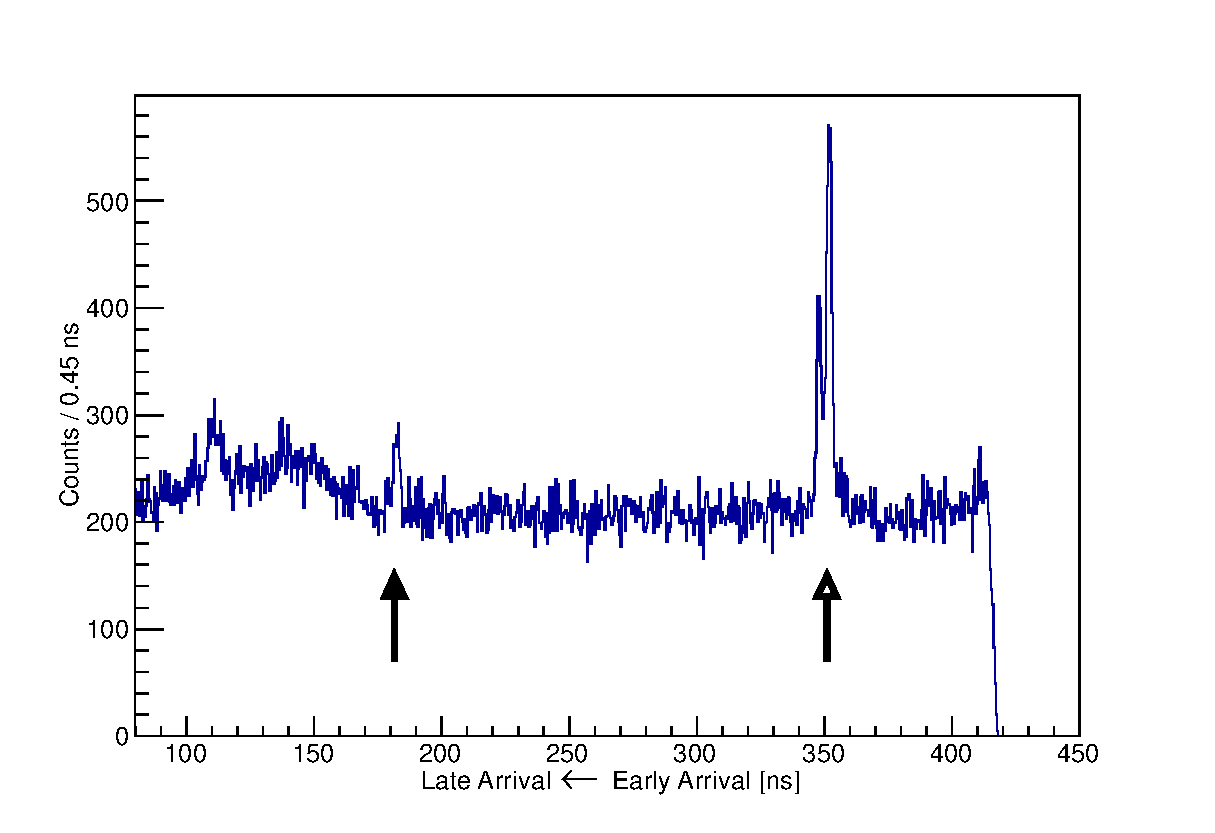
\includegraphics[width=0.5\textwidth]{figures/74Ge_sep_PS_barA.eps}
}
\subfloat[][]{
   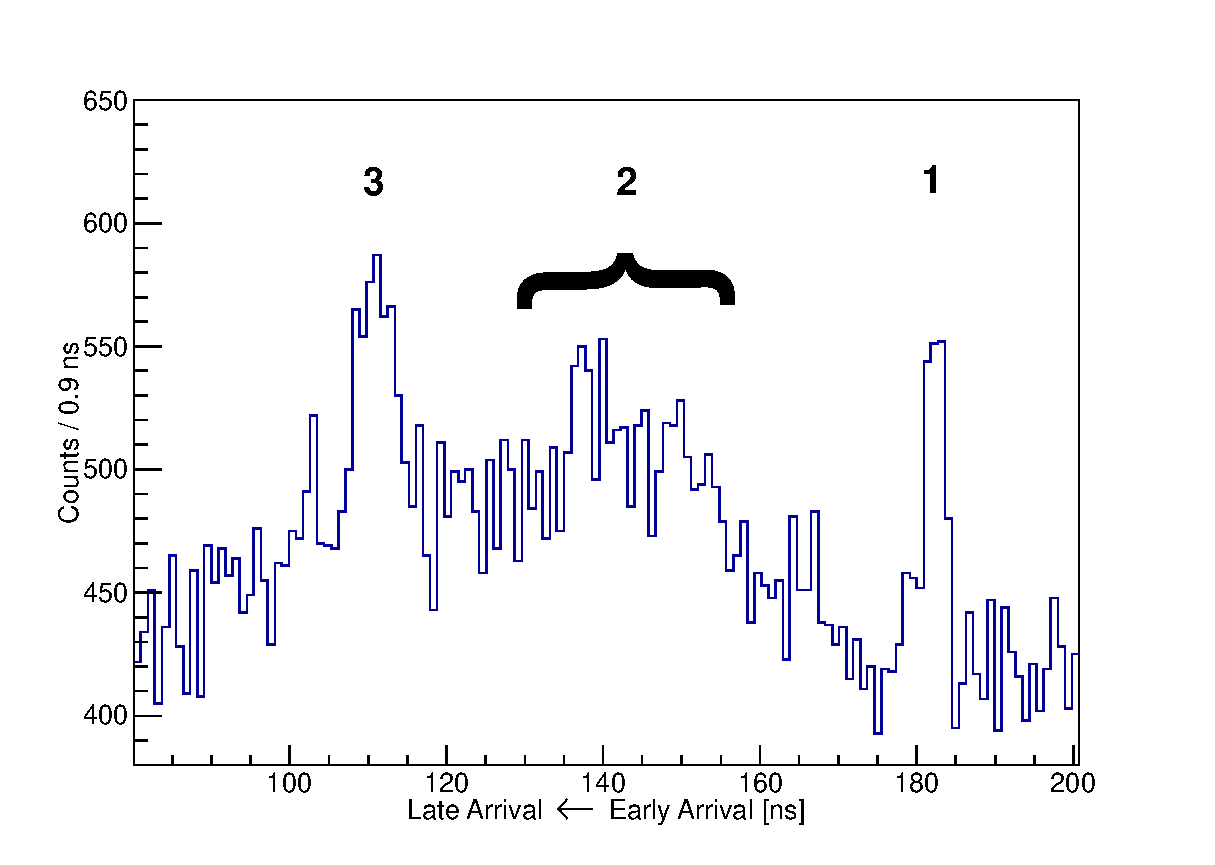
\includegraphics[width=0.5\textwidth]{figures/74Ge_sep_PS_barA_zoom.eps}
}
\caption{(a) A (time of flight) (TOF) spectrum from the forwardmost neutron detector bar (6.12$^{\circ}$) in the case of pulse-selected beam.  The reaction is $^{74}$Ge($^3$He,n)$^{76}$Se.  The ground-state neutron peak is indicated with a solid arrow and the $\gamma$-peak with a hollow arrow.  Note that the $\gamma$-peak is doubly-peaked, from beam hitting the target and then the beamstop.  (b) The neutron spectrum.  The ground-state neutron peak is indicated with a ``1'', the neutron continuum with a ``2''.  The other prominent peak, labeled ``3'', is due to oxygen contamination in the target.}
\label{fig:time}
\end{figure}
Another measurement important for analysis is the integrated light output at the top and bottom of a bar.  A geometric average of these, $\sqrt{E_tE_b}$, where $E_t$ and $E_b$ are the integrated light signal of the top and bottom PMT, respectively, is considered a measure of the neutron energy.  This is discussed further in {\sect}~\ref{sec:cuts}.  In this chapter, ``energy'' refers to the geometric average of the integrated light signals in a bar.  These signals, taken seperately, are not necessarily a measure of the energy of the event and will be referred to as ``light signals'' when used without averaging. 
% geometric average used twice, rewrite 

% a basic discussion of the data:
% TOF spectrum explained
% energy estimator

\section{Detector Efficiency}
\begin{comment}
deuterium, Mg, cuts
\end{comment}
\label{sec:efficiency}
The number of counts due to neutrons measured by the neutron detector scales linearly with the absolute cross-section of \reaction, corrected for the fact that not all the neutrons leave a signal in the detector.  The ratio of the detected neutron flux to the total neutron flux is called the efficiency of the detector and must be carefully determined as its error contributes directly to the systematic uncertainty of the extracted absolute cross-sections.

The efficiency of a plastic-scintillator-type neutron detector depends not only on the energy of the neutron, but also on the detector's size, shape, energy resolution, and detection threshold.  A Monte-Carlo code developed by Cecil \cite{Cecil_neutEfficiency} accurately calculates the efficiency of plastic scintillator detectors for a wide range of neutron energies and detector thresholds and was used to calculate efficiencies of the neutron detector for neutrons with energies of 10-28~MeV.  The efficiencies predicted by the Cecil code were verified against d(d,n) and \MgReaction measurements, both of which have well-known cross-sections.  Comparing the calculated efficiency to measured efficiency over a range inclusive of the neutron energies produced in \reaction gives confidence and also an estimate of the uncertainty in the efficiency.  The inputs required by the code are the density of the detector, its hydrogen to carbon ratio, the energy threshold applied to the data, and the interval over which the detector averages the light output, i.e., the resolution of the detector.  The plastic properties have been reported in {\tab}~\ref{tab:WLS_Kuraray}, and the threshold and resolution of the detector must be determined from the energy spectrum of the selected events from the experiment.  The cuts applied to the data are discussed in {\sect}~\ref{sec:cuts}.  An energy spectrum of the ground-state neutrons of any of the reactions studied can be produced by gating on the ground-state peak in the TOF spectrum.  The energy spectrum for the ground-state neutrons from \MgReaction is shown in {\fig}~\ref{fig:lowEnergyCut}. 
\begin{figure}[!htbp]
\centering
\includegraphics[width=0.8\textwidth]{figures/Lite_28MeV.eps}
\caption{The light curve of the 28~MeV neutron from \MgReaction is obtained by restricting the events to those in the ground-state peak window.  The data points shown in red are from the January dataset.}
\label{fig:lowEnergyCut}
\end{figure}
The width of the high-energy falloff gives the resolution of the detector, and the threshold can be determined by assuming the scale has a zero offset.  That this is a reasonable assumption is confirmed by the accuracy of the calculation.  

The efficiencies calculated using the above method must be checked for absolute accuracy of the prediction as well as accuracy of its predicted dependence on the energy of the detected neutron.  The reaction d(d,n), measured at beam energies near 9~MeV [cite], produces $\sim$12-MeV ground-state neutrons and is particularly useful because the neutron energy changes drastically as a function of angle, making it a useful check on the energy dependence of the Cecil prediction.  Additionally, empirical fits as described in [cite] provide excellent estimates of the absolute cross section in this energy region.  The agreement is excellent, as can be seen in {\fig}~\ref{fig:DeuteriumMatch}, which shows the prediction with and without correcting for neutron energy.  This result suggests that the Cecil code accurately adjusts the detector efficiency for neutron energy.  
\begin{figure}[!htbp]
\centering
\includegraphics[width=0.8\textwidth]{figures/deuteriumMatch.eps}
\caption{The prediction for d(d,n) (solid line) matches the data well when the efficiency is corrected for the neutron energy (red points).  The blue points represent the differential cross section where the efficiency is assumed to be the same at every angle despite a changing neutron energy.}
\label{fig:DeuteriumMatch}
\end{figure}

That the Cecil code appears to be successful in calculating the efficiency of the neutron detector for 12-MeV neutrons is encouraging, but neutrons from the ground states of \reaction will be $\sim$26~MeV.  A reaction with measurements of cross-sections for neutron energies in this range is \MgReaction.  While this reaction has not been measured at the beam energy of 16~MeV, which would produce a $\sim$28-MeV ground-state neutron, it has been measured at lower and higher energies as shown in {\fig}~\ref{fig:efficiencyCalib}.  The efficiency measured for the neutrons from this reaction provides a measurement very near the $\sim$26~MeV neutrons produced in \reaction and can be used to verify the absolute efficiency predicted by the Cecil code at neutron energies relevant to \reaction.  {\fig}~\ref{fig:efficiencyCalib} shows the consistency of the measured cross-section using that predicted efficiency.
\begin{figure}[!htbp]
\centering
\includegraphics[width=0.8\textwidth]{figures/magnesiumMatch.eps}
\caption{Checking consistency of efficiency calculation with \MgReaction.  This work (green) is consistent with measurements at surrounding energies (black).  The lines indicate spread due to statistical error.}
% circles - CCBA
% blue lines estimate of systematic error due to CCBA parameters
% squares are existing data
\label{fig:efficiencyCalib}
\end{figure}

\section{Experimental Parameters Related to the Cross Section}
\begin{comment}
current, tgt thickness (RBS), solid angle, dead time
go ahead and discuss errors while you discuss these quantities
\end{comment}

The differential cross section is the number of times a reaction occurred ($N_{reaction}$) normalized by the total number of particles incident on the target ($N_{beam}$), the number density of nuclei in the target ($n_{target}$), and the {efficiency of the detector}~($\epsilon$):
\begin{align}
\frac{d\sigma}{d\Omega} &= \frac{N_{reaction}}{N_{beam} \times n_{target} \times \epsilon}.
\label{eq:cross_section}
\end{align}
The efficiency $\epsilon$ of the detector includes the solid angle $d\Omega$.  Other quantities in the cross section that relate to the experimental setup are the number of particles incident on the target and the number density of nuclei in the target.

The three targets (\GeTargets and \Mg{26}) used in the experiments were provided by John Greene of Argonne National Laboratory (ANL).  The \GeTargets targets were evaporated onto a gold backing, while the \Mg{26} target is self-supporting.  The isotopic abundance and thickness of each target is shown in {\tab}~\ref{tab:targets}.  The target thicknesses were measured with an alpha-thickness gauge when they were made, and again at Hope College using Rutherford back-scattering (RBS).  RBS measurements are useful because they give information about the target composition, which must be assumed when calculating target thickness from alpha-thickness-gauge measurements.  The reported thicknesses were obtained by analyzing the RBS data with SIMNRA \cite{SIMNRA}, an RBS analysis software.  A sample of the fit for each target is shown in {\fig}~\ref{fig:RBS_sample}.  To estimate variations in target thickness, measurements were taken at several different positions on each target.
\begin{figure}[!htbp]
\centering
\subfloat[][]{
   \includegraphics[width=0.5\textwidth]{figures/76ge-4-holes.eps}
}
\subfloat[][]{
   \includegraphics[width=0.5\textwidth]{figures/76ge-4-adjusted.eps}
}
\caption{RBS data for the \Ge{76} target near the beamspot.  The plateau at low energies is due to pinholes in the target.  The plateau at high energies is due to small sections of the target with no \Ge{76} deposited on the gold surface.  The fit including the pinholes in the target is shown in (a).  The RBS spectrum, adjusted by subtracting the background due to pinholes, and its fit are shown in (b).  Fitting the RBS spectrum with and without adjusting for pinholes did not result in any significant differences to the predicted target composition or thickness.}
% move this to text, highlight features in plot
\label{fig:RBS_sample}
\end{figure}
\begin{table}[htp]
\centering
\begin{tabular}{lllll}
 & \multicolumn{2}{c}{$\alpha$-gauge ($\mu$g/cm$^2$)} & \multicolumn{2}{c}{RBS ($\mu$g/cm$^2$)} \\
\cline{2-3}\cline{4-5}
$^{74}$Ge & Au$_{\text{nat}}$ & 1011 & Au$_{\text{nat}}$ & 1001 \\
          & $^{74}$Ge & 1057 & $^{74}$Ge & 1016 \\
          &           &      & O$_{\text{nat}}$ & 9 \\[0.35cm]

$^{76}$Ge & Au$_{\text{nat}}$ & 1069 & Au$_{\text{nat}}$ & 1014 \\
          & $^{76}$Ge & 838 & $^{74}$Ge & 775 \\
          &           &      & O$_{\text{nat}}$ & 4 \\[0.35cm]

$^{26}$Mg & $^{26}$Mg & 791 & $^{26}$Mg & 685 \\
          &           &      & C$_{\text{nat}}$ & 10 \\
          &           &      & N$_{\text{nat}}$ & 43 \\
          &           &      & O$_{\text{nat}}$ & 52 \\
\end{tabular}
\caption{Target composition and thickness.  The $\alpha$-gauge measurements were performed at ANL and the RBS measurements at Hope College.}
\label{tab:targets}
\end{table}

To determine the absolute cross-section, it is also necessary to know the total number of \He{3} ions incident on the target for each dataset.  One monitor of the beam current is the charge collected by the Faraday cup.  A BaF$_2$ crystal outside the target chamber and a silicon detector inside the target chamber detect $\gamma$ radiation from beam incident on the target and scattered \He{3} beam, respectively.  Both these detectors monitor the product of the target thickness and the beam current.  Data from the silicon detector showed that the ratio of \GeTargets to gold does not change throughout the run and that the live charge collected by the Faraday cup scales with the back-scattered peak in the silicon spectrum.  The live charge can therefore be used to scale beam current between runs, making it possible to express \reaction cross sections in terms of the known \MgReaction cross section.

\section{Data Sets}
Two sets of \reaction data are available.  The first was taken in September of 2011.  A subset of this data was taken with no pulse selection due to hardware failure.  A second run in December of 2011 provided additional data, all taken with pulse selection.  During the December run, data were taken with the \GeTargets as well as \Mg{26} targets to provide an accurate normalization.  The data sets are summarized in {\tab}~\ref{tab:dataSets}.
\begin{table}[htp]
\centering
\begin{tabular}{llll}
            & & time.Live & Q.live \\
\hline
January     & PS 26Mg & 4645809 & 1043718 \\
	    & PS 76Ge & 7814211 & 2919101 \\
	    & PS 74Ge & 16379018 & 5312776 \\ \\

September   & PS 76Ge & 12616566 & 2872649 \\
	    & PS 74Ge & 11666670 & 2619116 \\
	    & NPS 76Ge & 27369635 & 15316275 \\
	    & NPS 74Ge & 11323947 & 10008757 \\
\end{tabular}
\caption{Data sets used in the analysis were obtained in two separate runs.  Data from the September run are both pulse-selected (PS) and non-pulse-selected (NPS).}
% too many digits - only need three or four
% need real units
% make labeling consistent
% 26Mg -> \Mg{26}
\label{tab:dataSets}
\end{table}

\section{Cuts}
\label{sec:cuts}
Four sets of cuts were applied to the data to generate a final data set.  The first cut verifies that the recorded event represents a real event rather than noise.  The next cut discards envents with too-low light signals, reducing the background due to $\gamma$ radiation.  Two final cuts reduce the muon background; one cut uses the veto, and the other eliminates events with light signals too large to be due to neutrons.

A true event should have energy above the noise level recorded in both top and bottom PMT's.  Additionally, the time signals from the top and bottom PMT's should be correlated.  A typical energy spectrum with no cuts applied and a typical scatter plot of timing from the top and bottom PMT are shown in {\fig}~\ref{fig:realEvent}.  Requiring correlated top and bottom timing signals is a cut that is applied to all bars in all final data sets.  The other requirement for a valid event is that the light signal be above the noise threshold.  An example of a light spectrum for a single bar and the noise threshold is shown in {\fig}~\ref{fig:realEvent}.
\begin{figure}[!htbp]
\centering
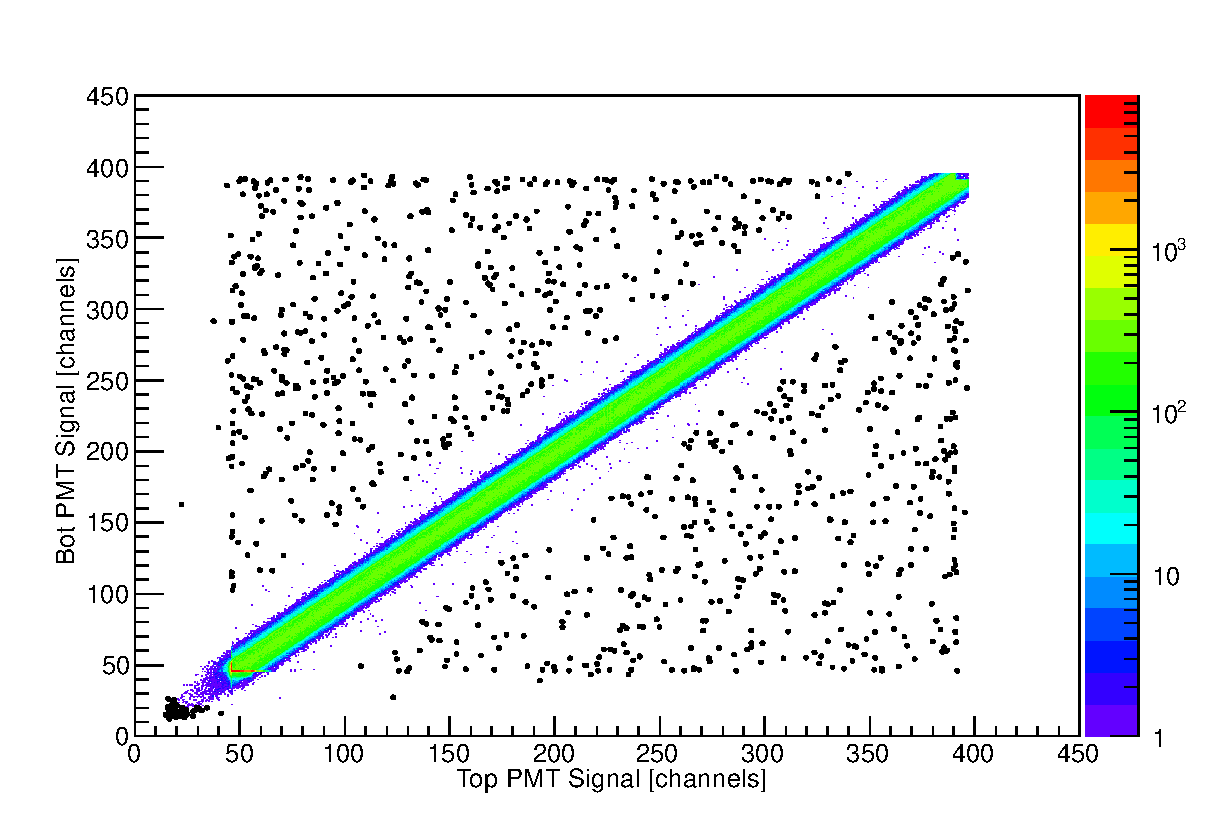
\includegraphics[width=0.8\textwidth]{figures/realTiming.eps}
\caption{Events with timing that is considered correlated are shown in color.  Black dots indicate events whose timing is not considered correlated.}
% unclear where the cut is
% change labels so it's clear the signals are timing signals
\label{fig:realEvent}
\end{figure}

% discussion of muon rejection begins here
Both the veto paddles and the bars of the neutron detector serve as a veto.  Veto paddle information is recorded as either ``true'' or ``false'' - true if a veto paddle fired during the event, false if it did not.  The bars of the neutron detector, in contrast, have more detailed information - time and light output.  While accidental coincidences are rare, the additional information provided by the bars of the neutron detector is used when these scintillators are used to veto.  For one bar of the neutron detector to veto another, both must have a valid signal and their average time must be similar.

A first approximation to determining whether or not an event is the result of a muon interaction is to require all but one bar in the neutron detector, as well as the entire veto, to be silent.  However, this would veto events that are spatially disconnected and could not possibly be due to a single muon.  To eliminate these unnecessary vetoes, we look at events that register signals in detectors with close spatial proximity, a ``veto group''.  One way to determine the appropriateness of increasing the size of a veto group is by looking at the energy spectrum of vetoed events.  Adding scintillator to a veto group that primarily eliminates muons results in an energy spectrum that has roughly equal numbers of high and low energy events, as shown in {\fig}~\ref{fig:muonVetoSpectrum}.  Material that does not veto primarily muon events will yield an energy spectrum that appears much more like the room background spectrum, heavily weighted towards lower energy events, as in {\fig}~\ref{fig:notMuonVetoSpectrum}.  These figures indicate that an appropriate group of material to use in the veto of a detector bar is the immediate, surrounding material.  Several samples of veto groups are shown in {\fig}~\ref{fig:vetoGroups}.  A separate cut to reject muons discards events that deposit energy above the maximum neutron energy deposition.    
\begin{figure}[!htbp]
\centering
\subfloat[][Energy spectrum of a neutron detector bar.  Entries in this histogram are from events having at least one correlated signal in the neutron detector and are likely to be muons.  Notice the high-energy-deposition peak at $\sim$ channel~3000 and its considerable height relative to the low-energy $\gamma$ background.  This low-energy background is dominant in non-muon events as in {\fig}~\subref{fig:notMuonVetoSpectrum}.]{
   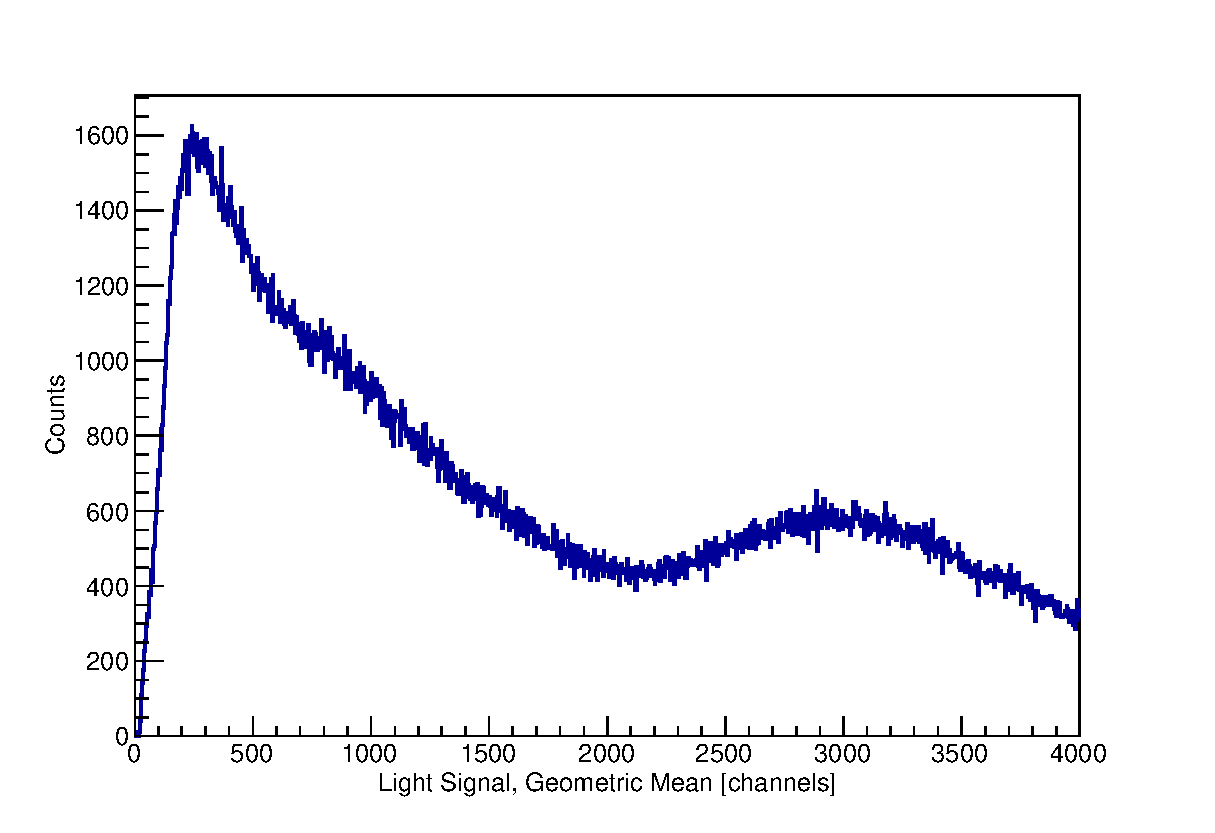
\includegraphics[width=0.45\textwidth]{figures/atLeastOneCorrelatedBar.eps}
   \label{fig:muonVetoSpectrum}
}
\hspace{8pt}
\subfloat[][Neutron detector bar energy spectrum.  These events have no correlation to other signals in the neutron detector and are unlikely to be due to muons.  While some high-energy depositions are visible, the spectrum is clearly dominated by the low-energy peak due to $\gamma$-radiation.]{
   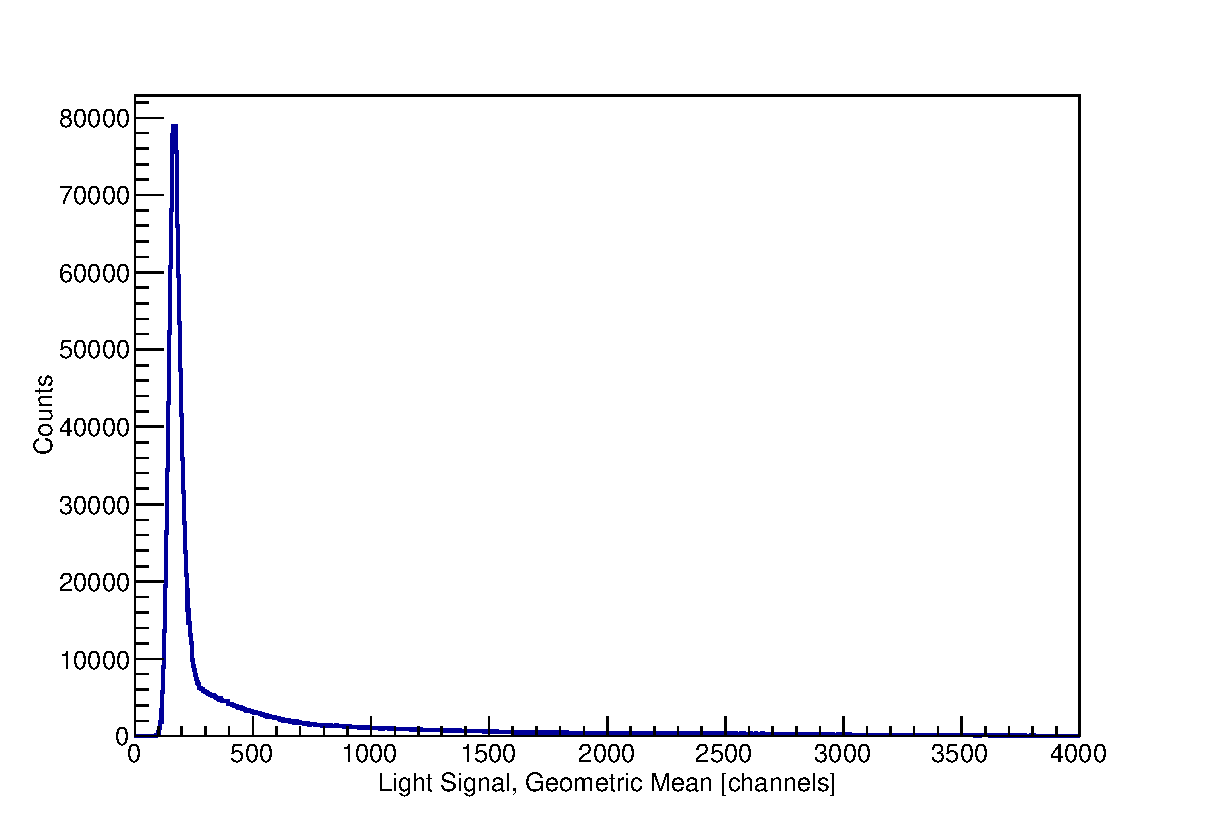
\includegraphics[width=0.45\textwidth]{figures/singleBar_noVeto.eps}
   \label{fig:notMuonVetoSpectrum}
} \\
\subfloat[][Sample groups of detectors chosen to veto bars in the neutron detector.  If the events in a neutron detector bar vetoed by a detector have an energy spectrum dominated by the low-energy $\gamma$-radiation, that detector is not used as part of the veto for that particular bar.]{
   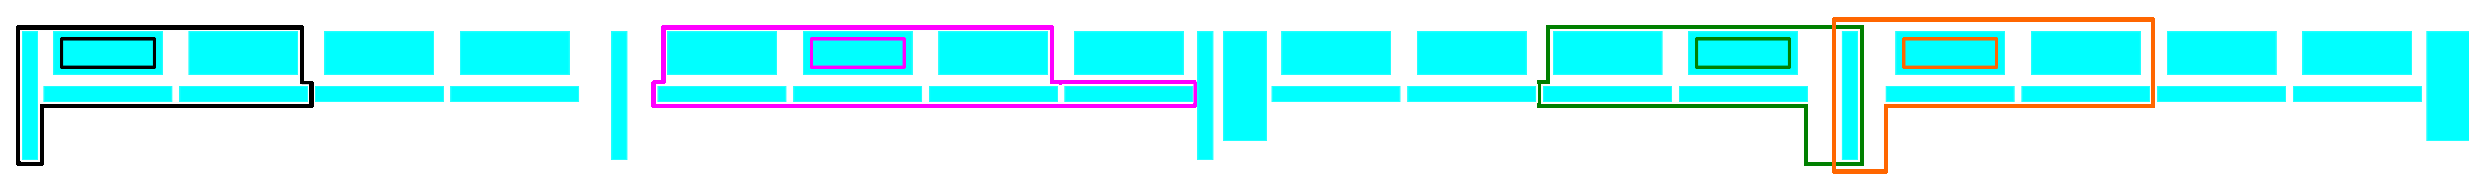
\includegraphics[width=1.0\textwidth]{figures/vetoGroups.eps}
   \label{fig:vetoGroups}
}
\caption{}
\label{fig:determineVetoGroups}
\end{figure}

% discussion of the low energy cut begins here
The final cut on the data sets is a lower energy cut to reduce the random background due to $\gamma$ radiation.  Placing a low-energy cut on the data is difficult becuase finding an estimator for the energy is not straight-forward.  It is appealing to argue that light loss due to attenuation must be exponential, and that an accurate estimator of the total deposited energy is the geometric mean of the top and bottom PMT signals:
\begin{equation}
\sqrt{Ae^{-\alpha x}\times Ae^{-\alpha (L-x)}} = \sqrt{A^2e^{-\alpha L}} = Ae^{-\alpha L/2},
\end{equation}
where $\alpha$ is a factor determined by the attenuation in the bar and $L$ is its length.  If this model of the signal attenuation is correct, the geometric mean should be position-independent.  This is not the case, as can be seen in {\fig}~\ref{fig:product_positionDependence}.  Furthermore, the position dependence is not often uniform even between the top and bottom PMT on a single bar, making it difficult to construct an average value.  Nonetheless, it is necessary to define a low-signal cut that is uniform for all the bars of the detector to avoid introducing significant systematic error into the final cross-section.
\begin{figure}[!htbp]
\centering
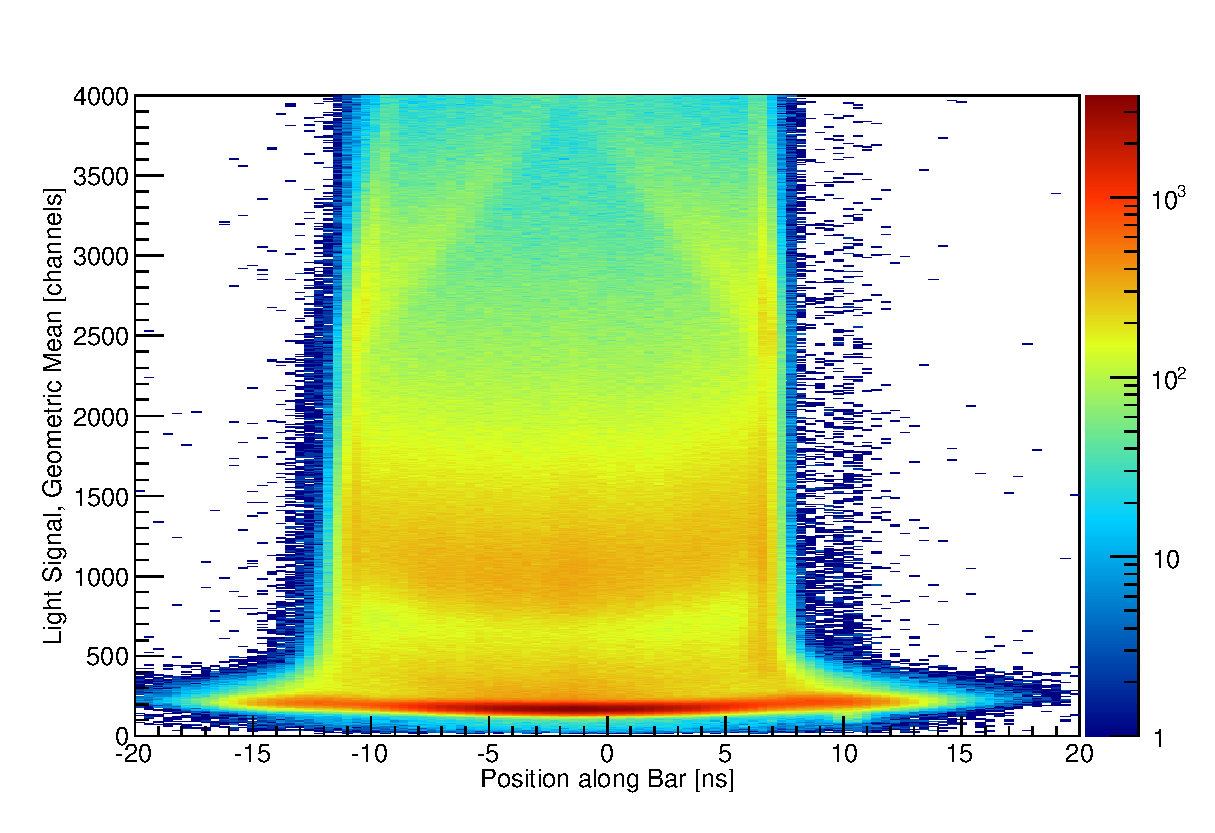
\includegraphics[width=0.8\textwidth]{figures/positionVSenergy.eps}
\caption{Position dependence of the geometric mean of the light signal of rejected events.  The band of events with light signals between $\sim$1000-1500~channels in particular demonstrates that the signal increases as it approaches the extremes of the neutron detector bar.  The events shown here are those that triggered the veto and are likely muons.}
\label{fig:product_positionDependence}
\end{figure}

Defining a position-dependent light signal cut on each PMT separately would be an ideal solution to these problems if the position dependence for a given energy were known.  While such a characterization of the PMT's for an arbitrary energy is not known, the muon events recorded by the detector do give the light signal as a function of position for one energy.  Due to the detector geometry, it is expected that the average path of the muons will be peaked at slightly more than 5~cm.  Simulations using the detector bar geometry and an angular distribution of $\cos^{1.3}{\theta}$ [CITE] (where $\theta$ is the normal from the surface vertical) confirm a well-defined peak in the muon path length. This most-likely path length manifests as a peak in the energy spectrum that depends only on the thickness of the bars and on the most likely angle of incident muons, both of which are the same for every bar in the neutron wall {need to state this is becuase they are MIP}.  A simulated energy spectrum is shown next to a real energy spectrum in {\fig}~\ref{fig:muonSpectrum}. 
\begin{figure}[!htbp]
\centering
\subfloat[][]{
   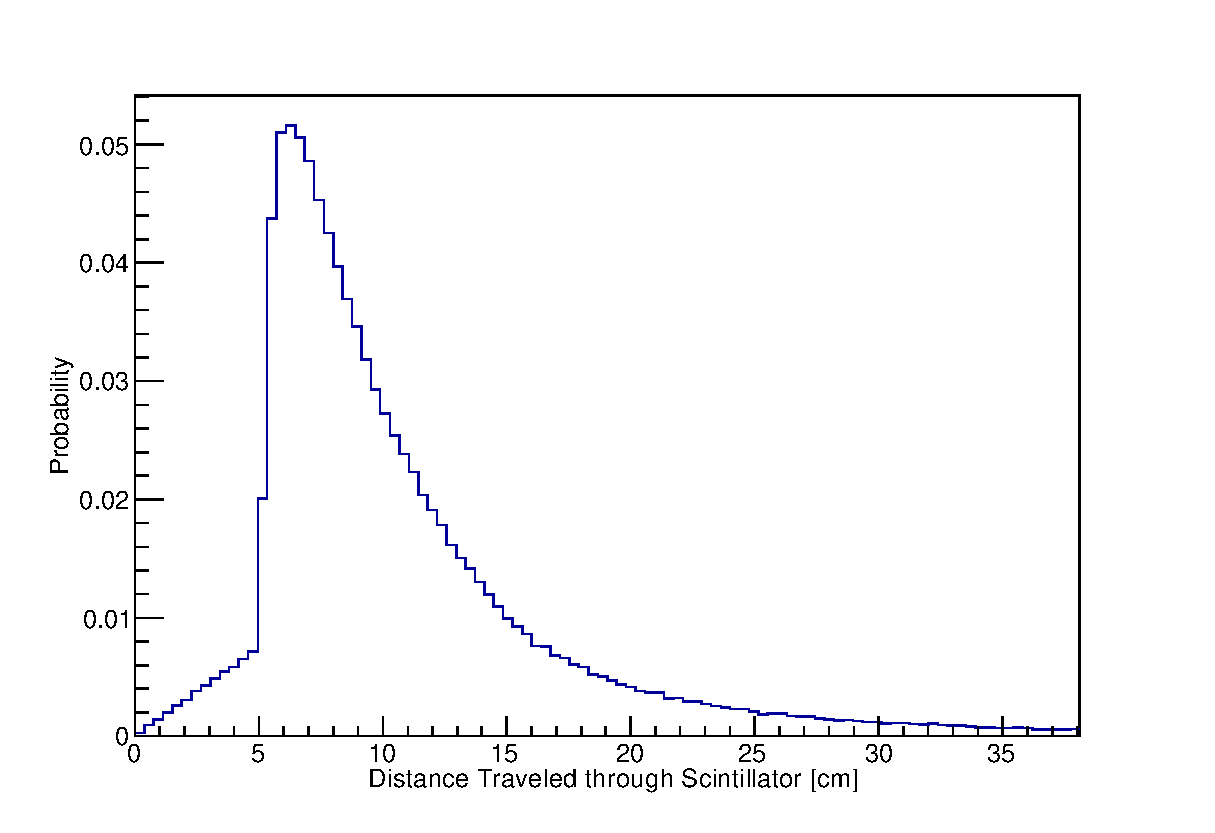
\includegraphics[width=0.5\textwidth]{figures/cosDist_distances.eps}
}
\subfloat[][]{
   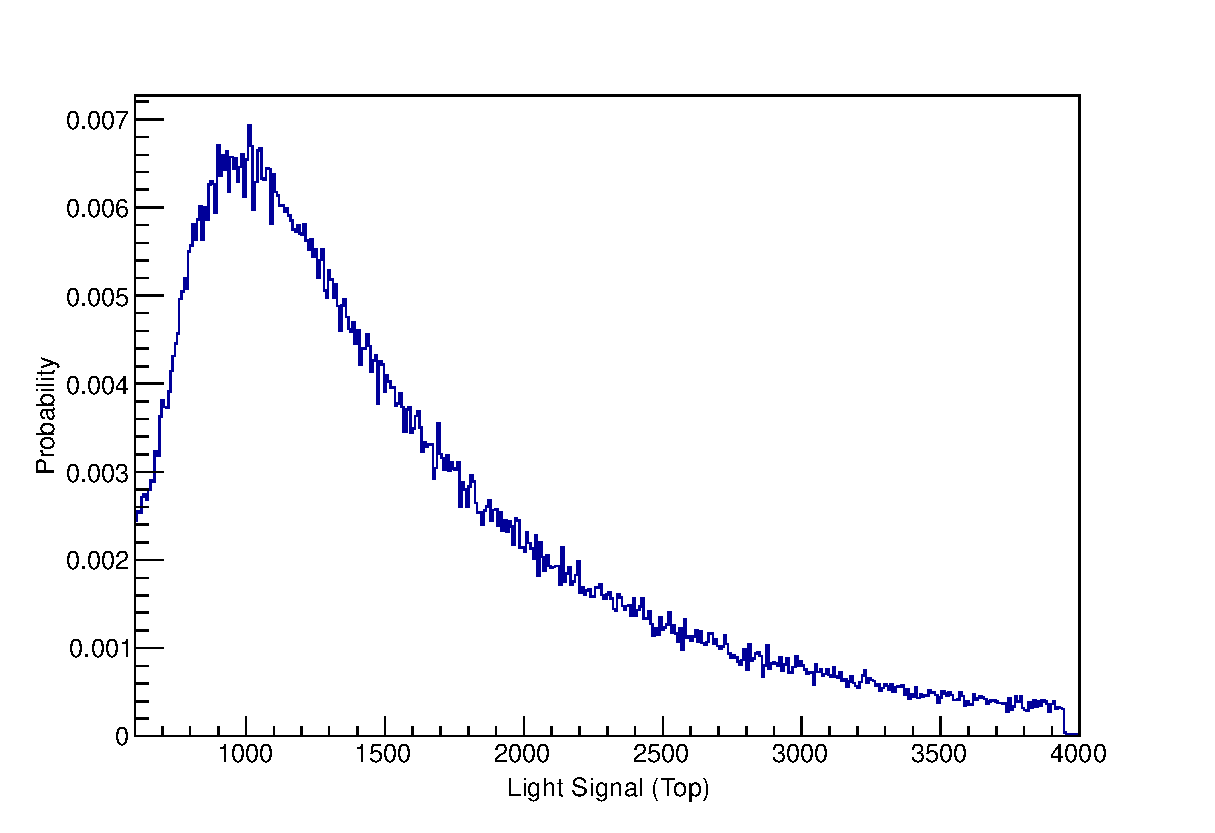
\includegraphics[width=0.5\textwidth]{figures/BarA_cosmics_centerSlice.eps}
}
\caption{(a) A simulation of path length of muons interacting in a detector with dimensions identical to those of the neutron detector bars.  Note the distinct peak. (b) Light signal of muon events near the center of the bar.  The peak in this distribution is believed to be the peak seen in the simulated spectrum.}
\label{fig:muonSpectrum}
\end{figure}
The peak of the light spectrum is assumed to represent the same energy and therefore to function as a calibration of the position dependence of the light signal due to the most likely muon energy deposition.  Fits to the location of the energy peak as a function of position are shown in {\fig}~\ref{fig:fits_pkVSpos}.
\begin{figure}[!htbp]
\centering
\subfloat[][The position dependence of the light signal from a single PMT.]{
   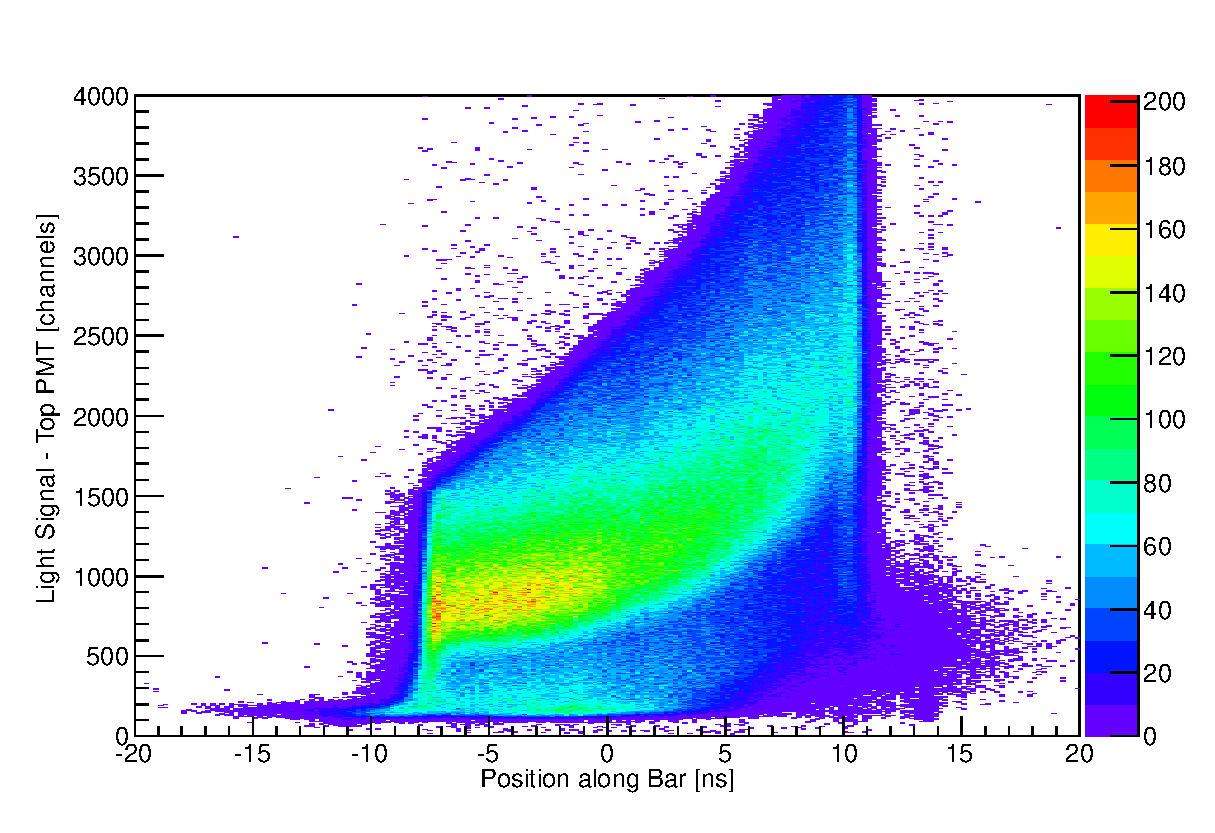
\includegraphics[width=0.8\textwidth]{figures/PMT_positionResponse.eps}
} \\
\subfloat[][The two-dimensional histogram shown in (a) is projected into a series of one-dimensional histograms.  The peaks of these histograms are determined by fitting with a Landau function.]{
   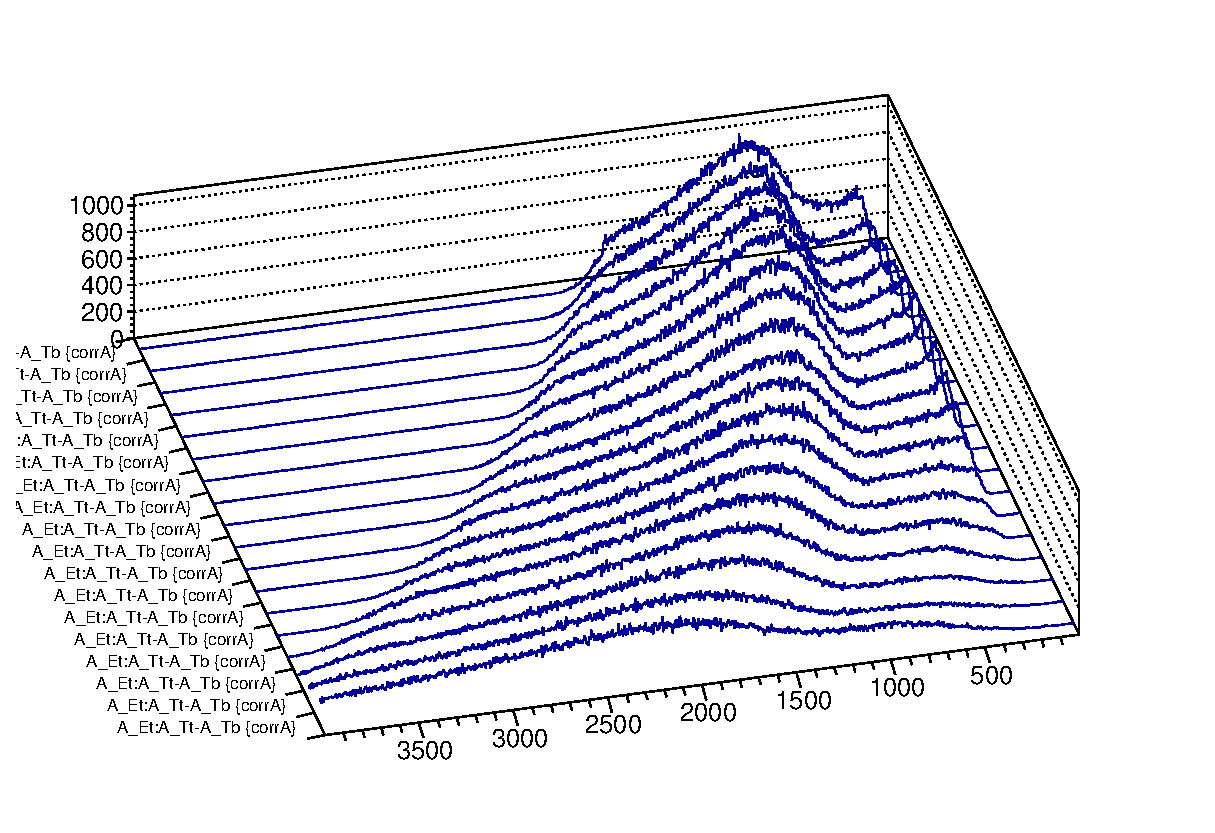
\includegraphics[width=0.45\textwidth]{figures/position_sliceGraphs.eps}
}
\hspace{8pt}
\subfloat[][A plot describing the curve which, when scaled, is used as the low-energy cut.  The points are determined from the histograms shown in (b).  Points at the extremes that do not follow the trend are used to determine the position cut.]{
   \includegraphics[width=0.45\textwidth]{figures/EnergyCutExample.eps}
}
\caption{}
\label{fig:fits_pkVSpos}
\end{figure}
Using the energy peak as a function of position itself as a lower energy cut results in an energy cut that is too high as can be seen in {\fig}~\ref{fig:highEnergyCut} {this is awkward, reword}.  Instead, these cuts are scaled to maximize the signal to noise ratio.  While high cuts discard more background, they also discard more neutrons, which are also likely to deposit a small amount of energy.  The minimum fractional error is acheived with a scaling factor that results in a reduction of the background by a factor of $\sim$1.4 (with all other cuts applied).  This is the case for every bar in the neutron detector; the fractional error as a function of the energy cut for the forwardmost bar is shwon in {\fig}~\ref{fig:signalToNoise}.  
\begin{figure}[!htbp]
\centering
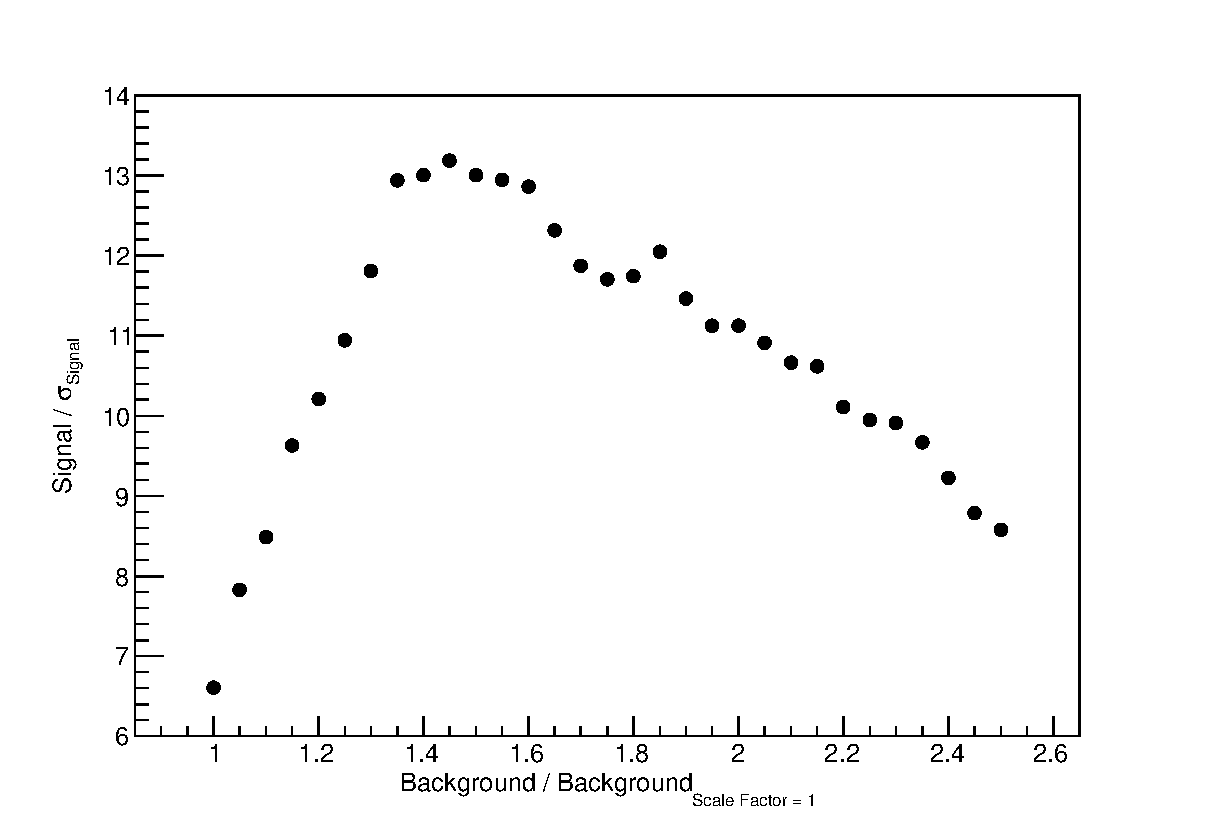
\includegraphics[width=0.8\textwidth]{figures/signalToNoiseCurveA.eps}
\caption{The ratio of the signal to its statistical error as a function of the energy cut.  The energy cut is parameterized as the background reduction to allow uniform scaling between bars.}
\label{fig:signalToNoise}
\end{figure}
Scaling ratios are determined by comparing the background to that of the initial cut as in {\fig}~\ref{fig:scalingFactor} to obtain uniform scaling from bar to bar.  
\begin{figure}[!htbp]
\centering
\subfloat[][Applying a scaling factor to the cut determined as in {\fig}~\ref{fig:fits_pkVSpos} is measured relative to the background obtained with the unscaled cut.  The effect of the highlighted scaling factors is shown in {\fig}~\subref{fig:highEnergyCut}.]{
   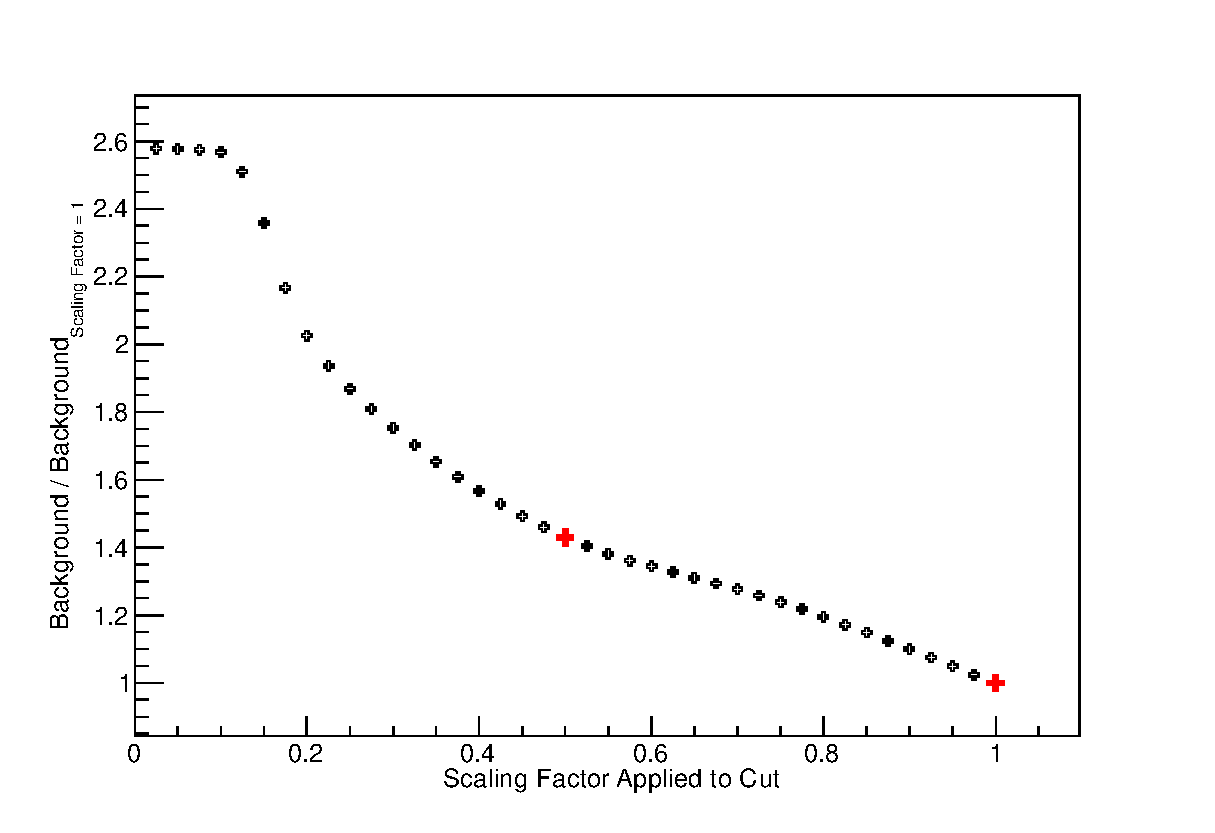
\includegraphics[width=0.45\textwidth]{figures/scalingFactor.eps}
   \label{fig:scalingFactor}
% get rid of this figure and replace with optimization figure
}
\hspace{8pt}
\subfloat[][Without applying a scaling factor to the cut determined as in {\fig}~\ref{fig:fits_pkVSpos}, the neutron signals are nearly lost.  Scaling the cut by $\sim$0.5 results in a reasonable signal to noise ratio.]{
   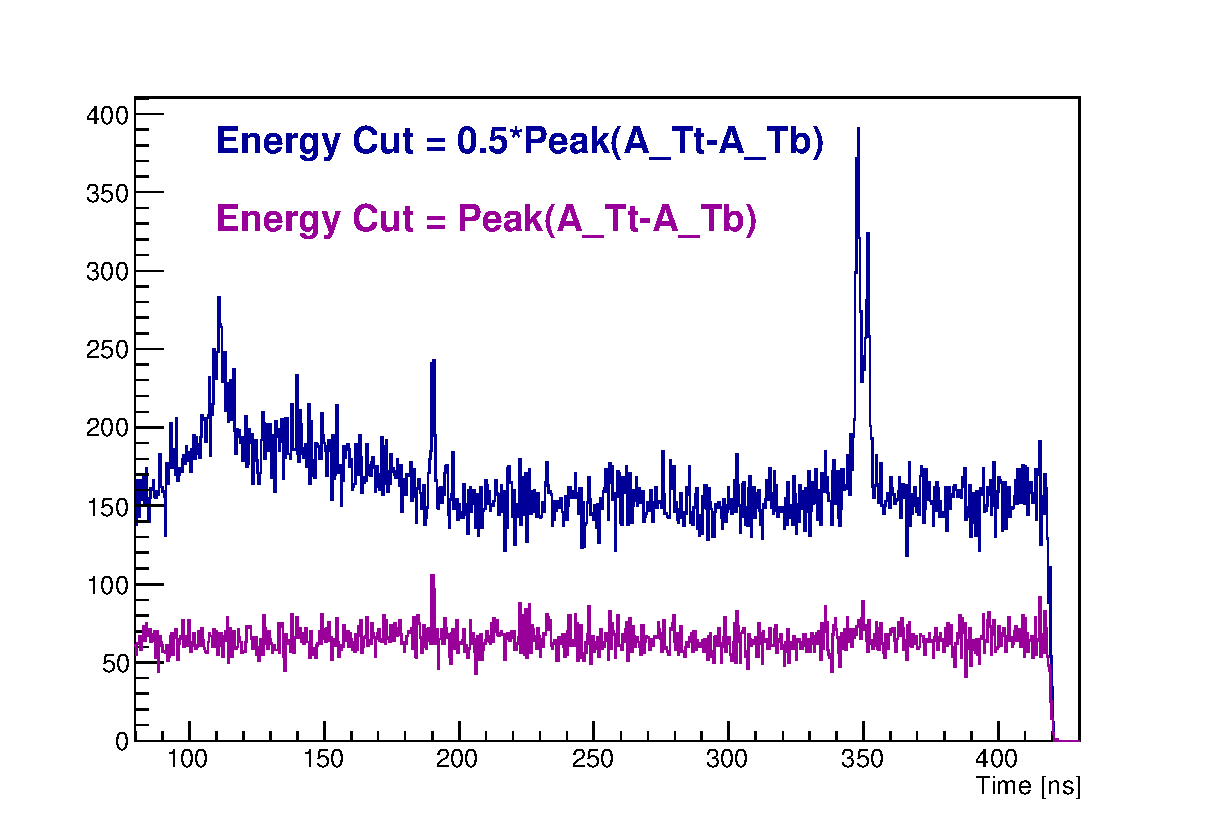
\includegraphics[width=0.45\textwidth]{figures/needLowerCut.eps}
   \label{fig:highEnergyCut}
}
\caption{}
\label{fig:scalingFactorEffect}
\end{figure}
An additional concern is that simply scaling the energy cut may not provide an accurate position dependence.  No distinct feature exists at lower energies, making this difficult to check directly.  However, the position distribution of rejected events with these scaled energy cuts is flat as seen in {\fig}~\ref{fig:flatPositionSpectrum}, suggesting that the position dependence at the most-likely deposited energy for muons is a reasonable approximation for lower-energy events.
\begin{figure}[!htbp]
\centering
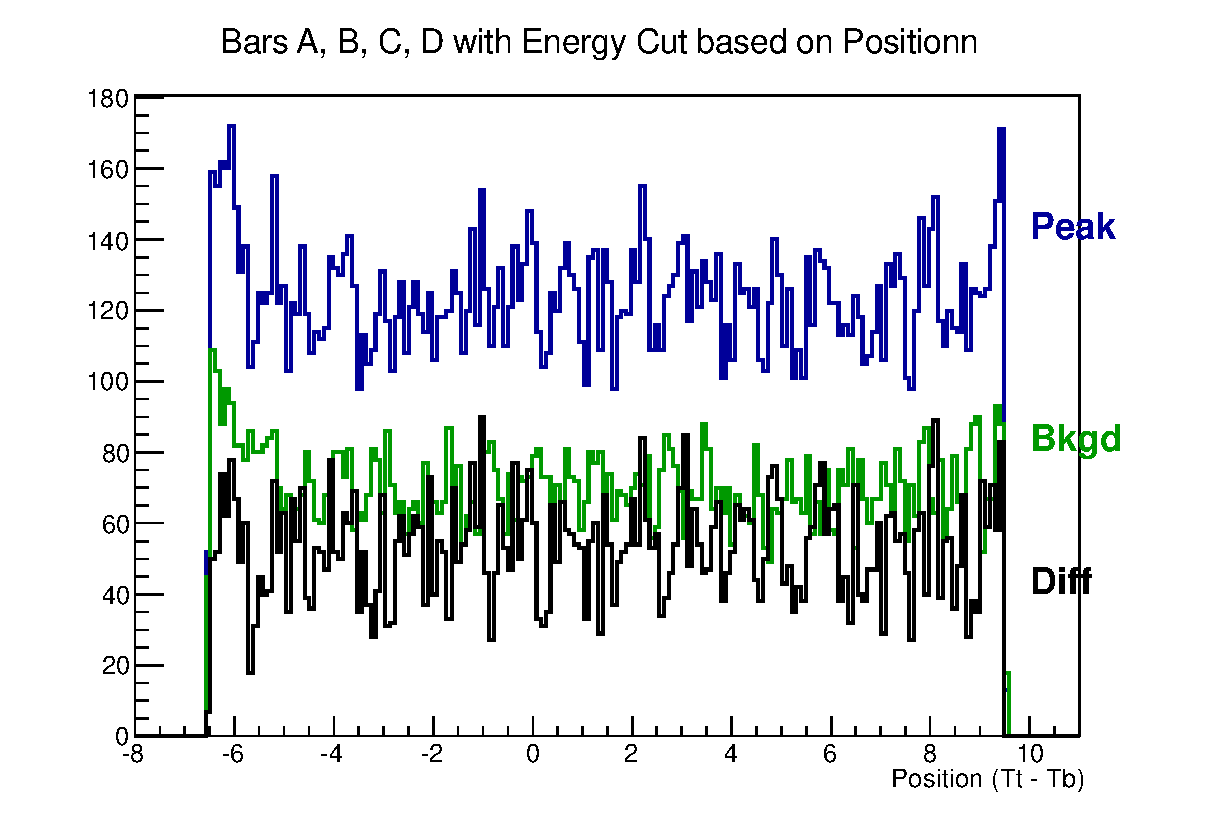
\includegraphics[width=0.8\textwidth]{figures/PositionSpectrum.eps}
\caption{A histogram of event position with a lower energy cut based on position.  The difference between the position spectra of the region around the ground state neutron peak (blue) and a background region with the same number of bins (green) is shown in black.  That this resulting position spectrum is flat indicates that the position dependence of the cut is appropriate.}
% rebin
% make sure spectra are clearly visible
\label{fig:flatPositionSpectrum}
\end{figure}

\section{Ground State Cross-Section}
\begin{comment}
two data sets
- pulse selection
- no pulse selection

background
- gamma peaks - do not overlap with neutron peak
- other neutron peaks - ??
- randoms - background in both data sets
- continuum - more important in non-pulse-selected data

extracting counts 
- pulse selection
- no pulse selection
\end{comment}

To extract the counts due to the ground-state neutrons one can sum the counts in the region of the peak and subtract the estimated background:

\begin{equation}
\text{S = P - B},
\label{eq:counts}
\end{equation}
where S is the extracted number of signal counts, P is the number of counts in the signal region, and B is the number of estimated background counts.  The error associated with $S$ is
\begin{equation}
\sqrt{\sigma_{P}^2 + \sigma_{B}^2}
\label{eq:errDef}
\end{equation}
where both $P$ and $B$ can be understood as a random variable with error $\sqrt{P}$ and $\sqrt{B}$, respectively.

The primary challenge is finding an accurate way to estimate the background that reduces the error of the extracted counts.  As can be seen in {\fig}~\ref{fig:PSvsNPS}, the background of the pulse-selected data is much simpler than that of the non-pulse-selected data.  Analysis of the datasets taken with pulse selection is straightforward and will be discussed first.  Without pulse selection, the neutron peak is superimposed on background from previous neutron bunches.  Extraction of neutron counts from these data will be discussed second.
\begin{figure}[!htbp]
\centering
\subfloat[][]{
   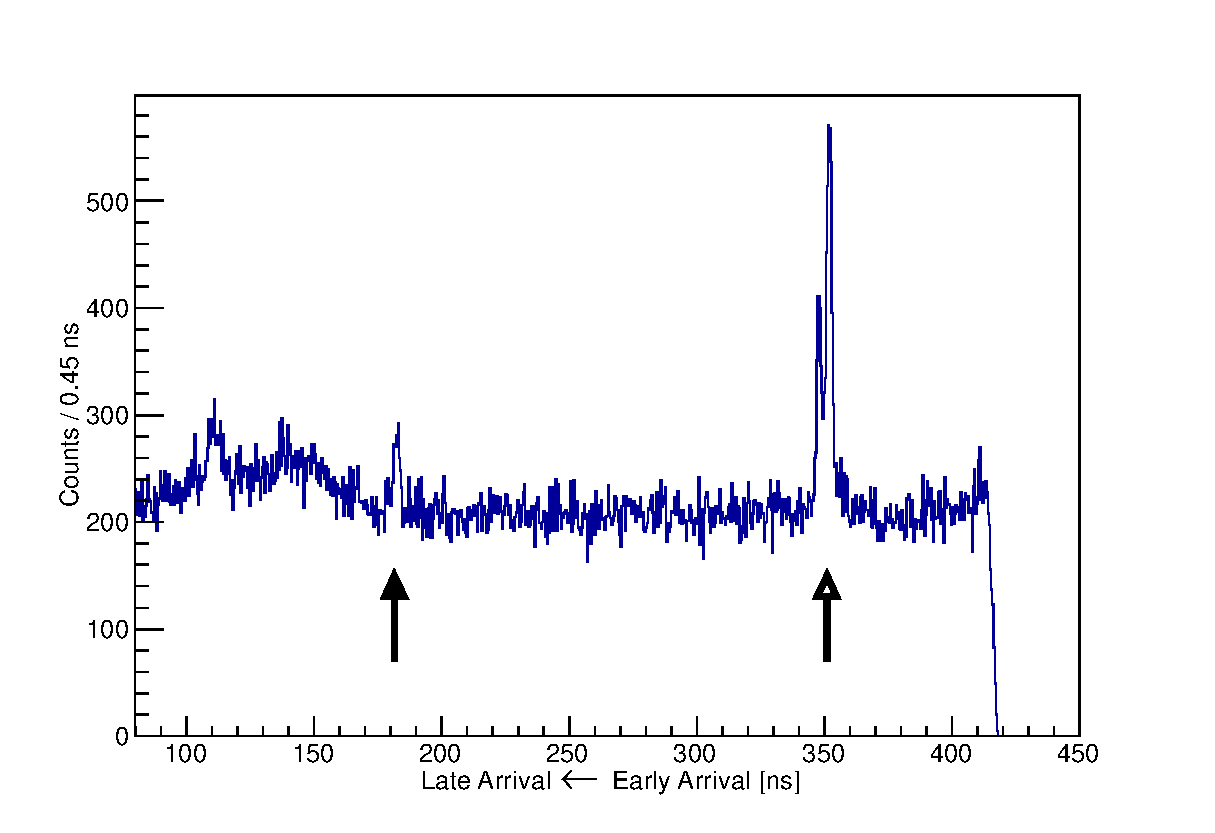
\includegraphics[width=0.5\textwidth]{figures/74Ge_sep_PS_barA.eps}
}
\subfloat[][]{
   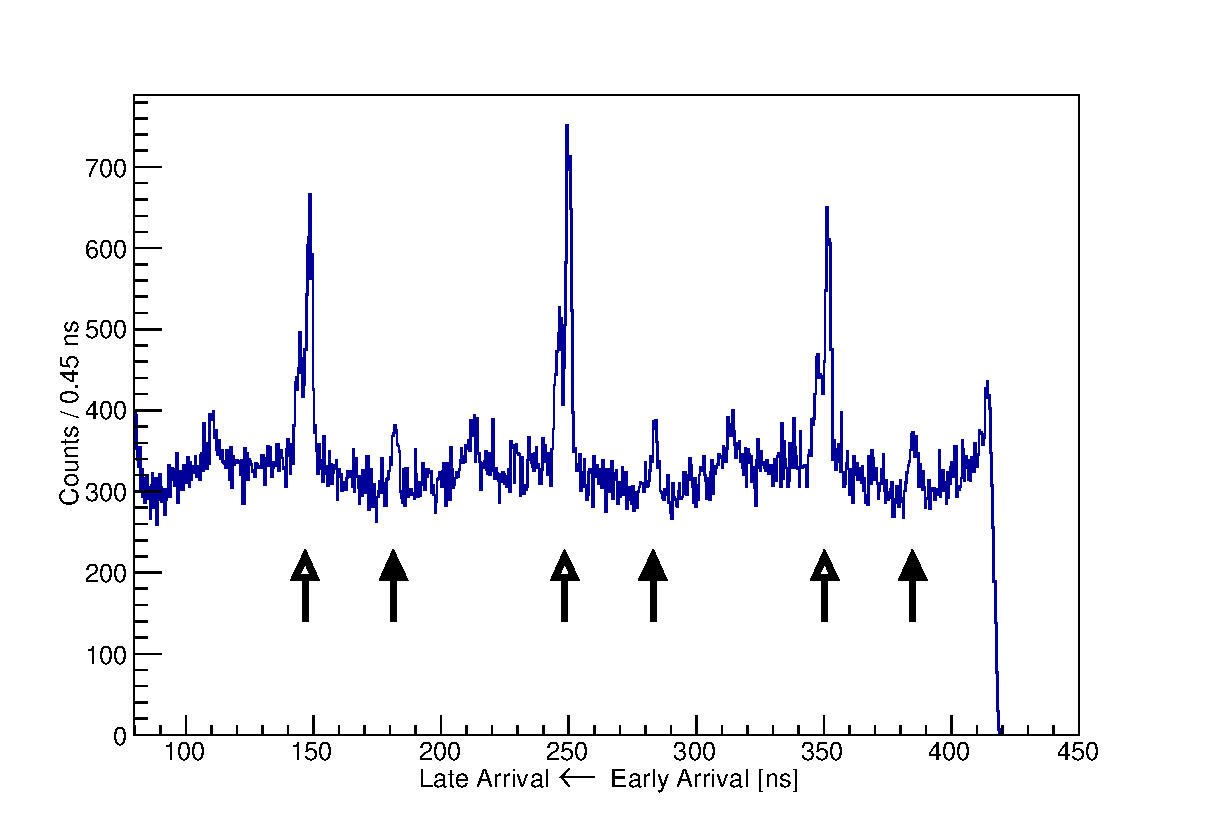
\includegraphics[width=0.5\textwidth]{figures/74Ge_sep_NPS_barA.eps}
}
\caption{The TOF spectrum of the forwardmost neutron detector bar (6.12$^{\circ}$) in the case of pulse-selected beam (a) and non-pulse-selected beam (b).}
\label{fig:PSvsNPS}
\end{figure}

\subsection{Pulse-Selected Data}
\label{sec:PS_data}
In the case of the pulse-selected data, the background in the region of the ground-state peak consists of flat, random background and the high-energy tail of the neutron continuum.  The $\gamma$-ray peaks are far away from the neutron peak and have no effect.  The random background is well-constrained in the region between the ground-state neutron peak and gamma peak.  The neutron continuum is due to multiple direct reactions and can only contribute to the background of the ground state neutron peak due to detector resolution.  Limits on the contribution of the continuum will be discussed later.  For now, we focus on the simplest contribution to the background, the flat distribution due to random radiation.

In the case of the pulse-selected data, estimating the background is done by fitting the flat background.  In general, the signal $S$ is calculated by subtracting the estimated background $B$ from the number of counts $P$ in the peak region.  If the flat background region is fit to obtain $n$, the number of counts per bin, the extracted counts become
\begin{equation}
S = P - B = P - n\times N_b,
\end{equation}
where $N_b$ is the number of bins in the peak region.  The error on the extracted counts is then
\begin{equation}
\sqrt{N_{\text{peak}} + {\sigma}_n^2\times N_b}.
\end{equation}
The error on the background no longer behaves like that of a random variable because $\sigma_n\sim\sqrt{\frac{n}{N_b}}$.  In the \reaction data sets, the error contribution ${\sigma}_n^2\times N_b$ is of order unity and is therefore negligible compared to the statistical error associated with the number of counts in the peak region.  Using an estimate of the background based on as many bins as possible, then, results in an error of approximately $\sqrt{P}$.

Thus far, the primary source of uncertainty is the statistical uncertainty associated with the number of counts in the peak region.  The uncertainty introduced by the continuum must also be estimated.  A neutron continuum is clearly visible for all reactions.  In the \Si{28} case, the continuum is well-separated from the ground-state neutron peak, but for \Se{76} and \Se{78}, it is unclear if the continuum contributes to counts in the peak region.  The \reaction data have the potential to be influenced by counts from the continuum because the continuum is much closer to the ground-state neutron peak than for \MgReaction and also because the integration window must be wide enough to include both the ground and first excited states.  To estimate the contribution of the continuum to the peak region, it is fit with a Gamma Distribution, shown in {\fig}~\ref{fig:BetaGamma}.  
\begin{figure}[!htbp]
\centering
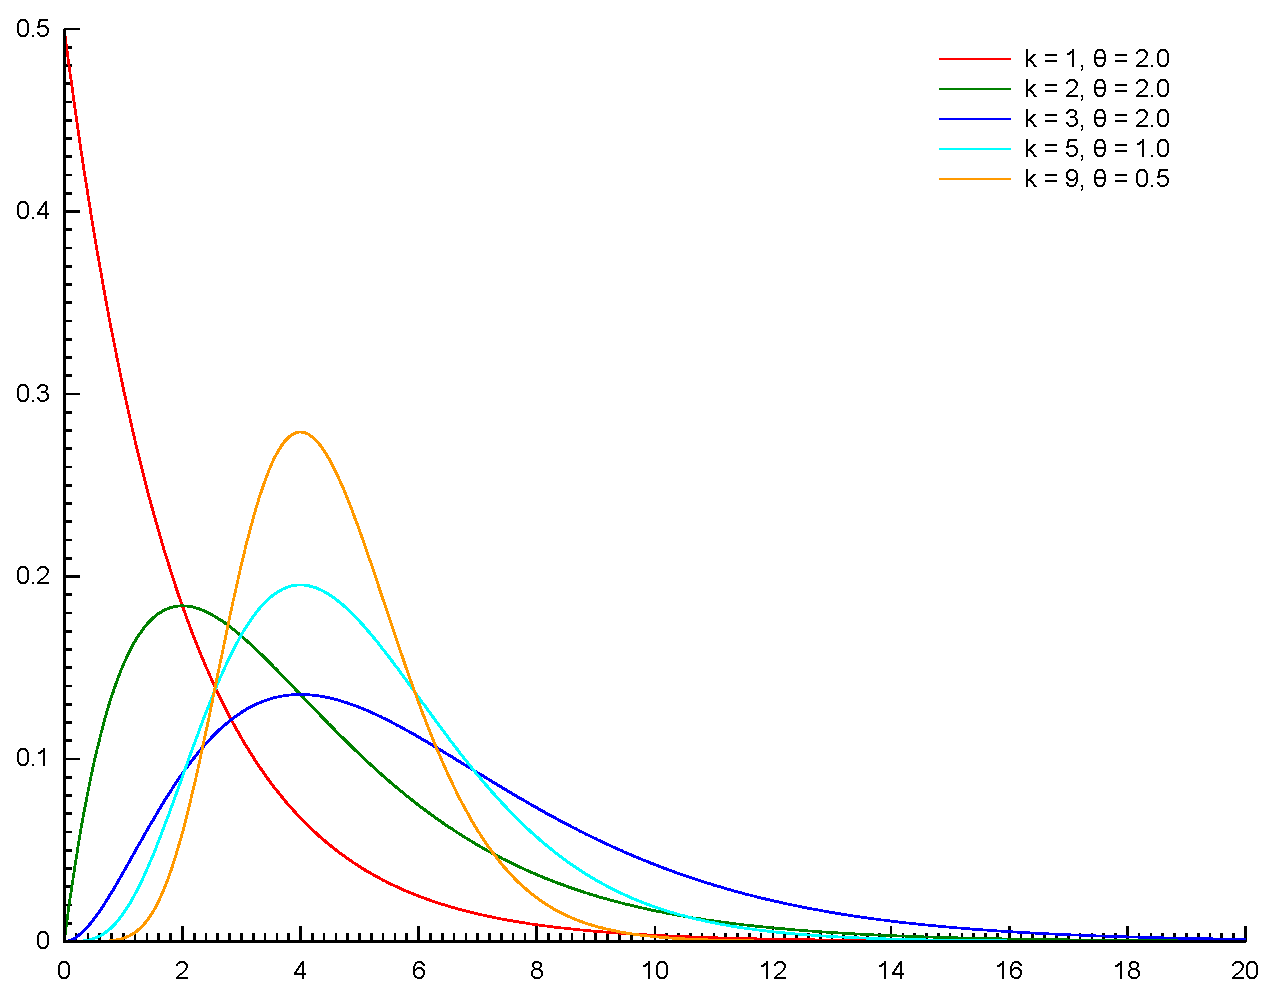
\includegraphics[width=0.8\textwidth]{figures/Gamma_distribution_pdf.eps}
\caption{The Gamma Distribution for various shape parameters \cite{wiki_Gamma}.  The distribution falls to zero at the origin; it is this property that makes this distribution a candidate model for the neutron continuum.}
\label{fig:BetaGamma}
\end{figure}
This is an appropriate functional model because neutrons populating the continuum cannot have an energy greater than the ground-state neutron, and so its endpoint cannot extend past the center of the ground state neutron distribution; the Gamma Distribution is non-zero only on a semi-infinite range.  The pulse-selected data set, however, does not constrain the tails of these functions well because the timing spectrum is not complete.  The non-pulse-selected data can help better constrain the fits in this region.

For the same bar, the pulse-selected spectrum should have the same shape as the non-pulse-selected data.  Fitting to the pulse-selected and non-pulse-selected histogram simultaneously greatly improves the fit because each bar of the neutron detector should measure the same beam-related spectrum for different runs, making it possible to model the non-pulse-selected spectrum as a shifted, scaled copy of the pulse-selected data.  The model used for the pulse-selected data is
% equation for pulse-selected spectrum
\begin{equation}
f_{PS} = g(x;\alpha,\beta) + Gaus_1 + Gaus_2 + Gaus_3 + DoubleGaus + Const_{PS}
\end{equation}
where $g(x;\alpha,\beta)$ is the Gamma Distribution; $Gaus_1, Gaus_2, Gaus_3$ are Gaussian Distributions describing prominent peaks in the continuum {g.s. not in continuum}; and $DoubleGaus$ models the $\gamma$-peak.  These terms are needed to ensure a good overall fit and their parameters are described in {\fig}~\ref{fig:continuumModel}.  The non-pulse-selected data can be modeled by shifting the pulse-selected model by the interval between bunches $\tau$:
% equation for non-pulse-selected spectrum
\begin{equation}
R\times(f_{PS}(t) + f_{PS}(t+\tau) + f_{PS}(t+2\tau)) + Const_{NPS},
\label{eq:NPS_model}
\end{equation}
where $R$ is the ratio of total beam on target between the pulse-selected and non-pulse-selected runs.  Such a fit converges well and shows that the neutron continuum contributes at most ??\% to the extracted counts in the ground-state neutron peak.  

The method used to extract the counts in the ground-state neutron peak is a direct summing of the counts from the peak region followed by subtraction of the estimated flat background from a linear fit.  The estimated error is the statistical error of the sum of the peak region and the systematic error of including counts from the continuum.  The results are plotted in {\fig}~\ref{fig:PS_angularDistribution}.
\begin{figure}[!htbp]
\centering
\subfloat[][]{
   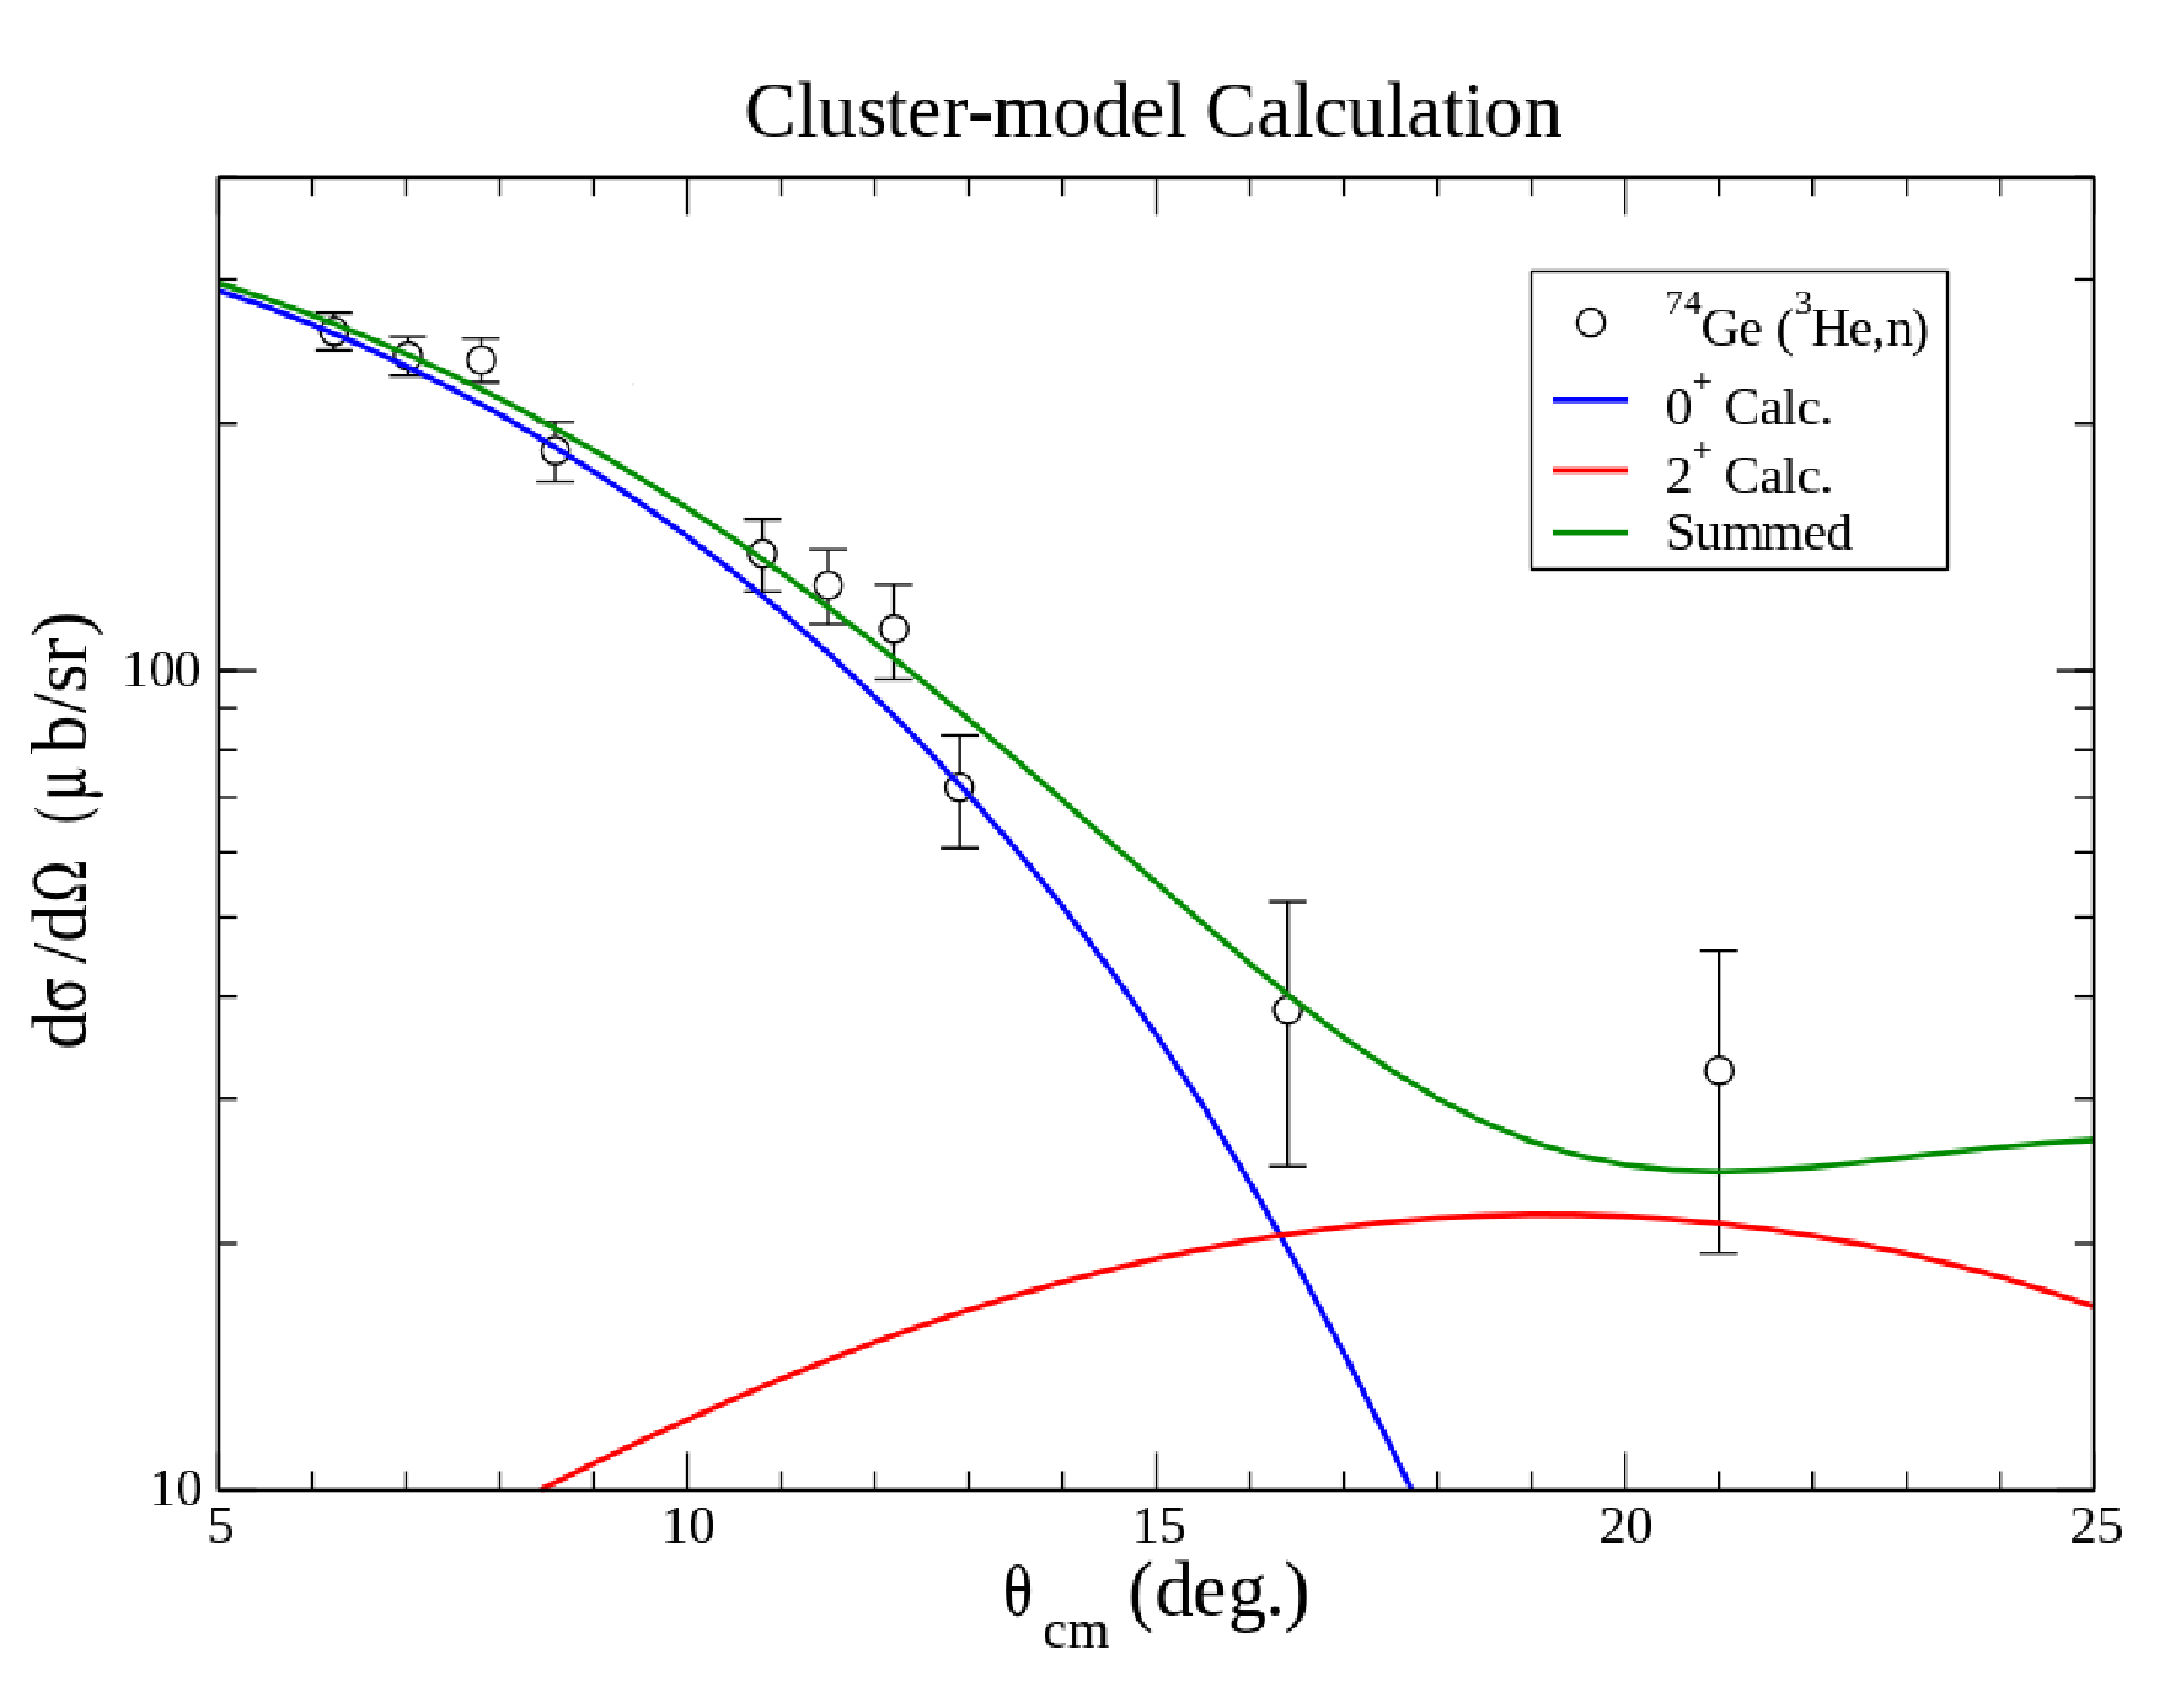
\includegraphics[width=0.5\textwidth]{figures/74Ge_angularDist.eps}
}
\subfloat[][]{
   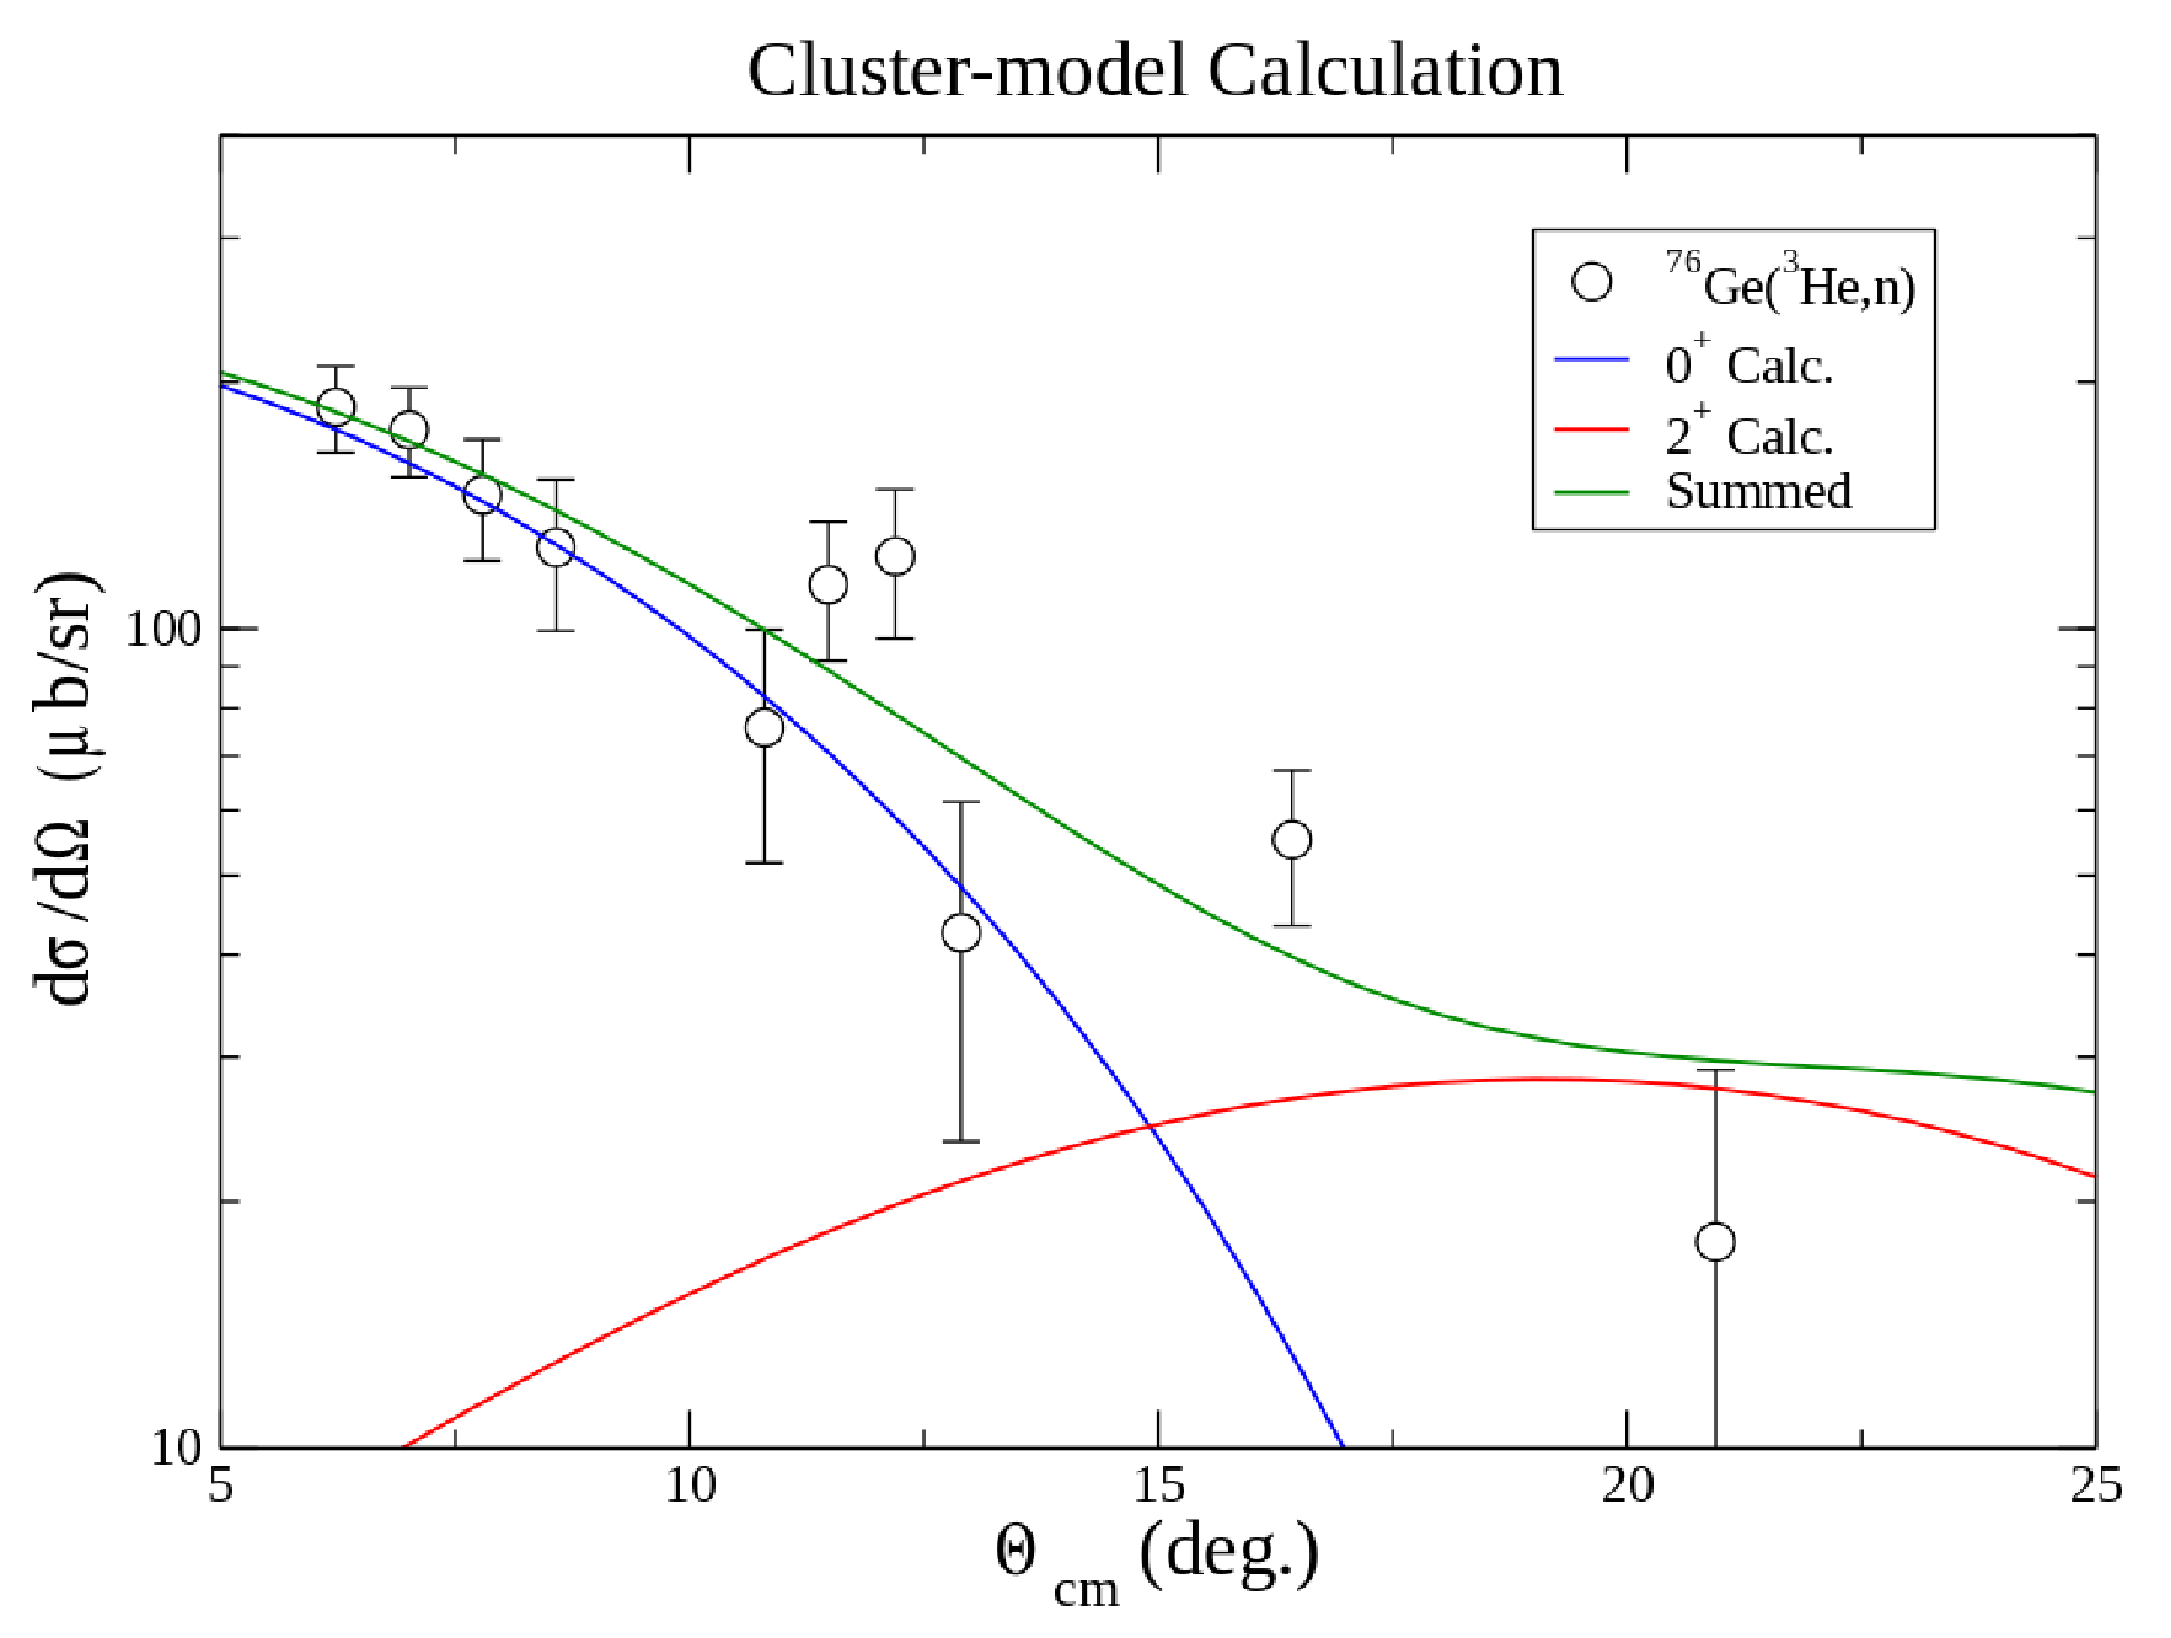
\includegraphics[width=0.5\textwidth]{figures/76Ge_angularDistribution.eps}
}
\caption{(a) The angular distributions of the ground-state first excited state $^{74}$Ge($^3$He,n)$^{76}$Se and (b) $^{76}$Ge($^3$He,n)$^{78}$Se (b).  In each graph, the two back-angle measurements are four-bar averages.  Because the timing resolution did not allow clear separation of the ground and first excited states, the integration window included both.  The data are well-described by the sum of the two states.}
% edit figure so it JUST shows the data
% edit caption so it mentions calcs discussed later 
\label{fig:PS_angularDistribution}
\end{figure}

%A dedicated fitter may begin to wonder if there are as-yet-unused constraints that could provide an even more robust fit that would ensure a convergent fit for all angles.  One additional constraint concerns the ratio between the two datasets.  This ratio scales the amount of beam seen by one bar during the two data runs.  But each bar should see the same ratio!  Fitting all the bars simultaneously will provide a much-improved ratio.

\subsection{Data with No Pulse Selection}
With pulse selection, the region between the ground-state neutron peak and $\gamma$-ray peak is solely due to the random background signal and can be fit with a constant to within ??\%.  With no pulse selection, the neutron peak is superimposed on background from the previous bunch.  Fitting this spectrum by itself introduces significant uncertainty in the height of the continuum because the flat background is not well-constrained by any portion of the spectrum.  The fit described above is a poor estimate of the background in the non-pulse-selected data because a wide range of shapes describing the neutron continuum and random background produce good fits but very different estimated background in the ground-state neutron peak region.  Additionally, it becomes difficult to introduce enough peaks to accurately reproduce the shape of the background without making the fit unable to converge because there are too many independent variables.  Another method for extracting counts due to a signal is side-band subtraction, where two regions on either side of the signal region, each with half the channels of the signal region, are chosen to estimate the background.  The accuracy of sideband subtraction, however, depends on a background that does not change rapidly near the signal region. 

Rather than estimating the background by fitting the non-pulse-selected spectrum with a function or with side-band subtraction, using the pulse-selected data itself as a template for the non-pulse-selected data is more accurate.  If the pulse-selected spectra are modeled as
\begin{equation}
Beam_{PS} + Const_{PS},
\end{equation}
then the non-pulse selected spectra can be generated as in {\eqn}~\ref{eq:NPS_model} by replacing the function estimates of the pulse-selected data with a Kernel Density Estimate [CITE] based on the data in the histogram.  

Extraction of the ground-state neutron counts is done not by subtracting an estimated background from the total counts in the peak region, but rather by applying the ratio of signal to background, $R/Const_{NPS}$, to the total counts.  The results of the fits can be seen in {\fig}~\ref{fig:NPS_fits} and the final angular distribution in {\fig}~\ref{fig:NPS_angularDistribution}.
\begin{figure}[!htbp]
\centering
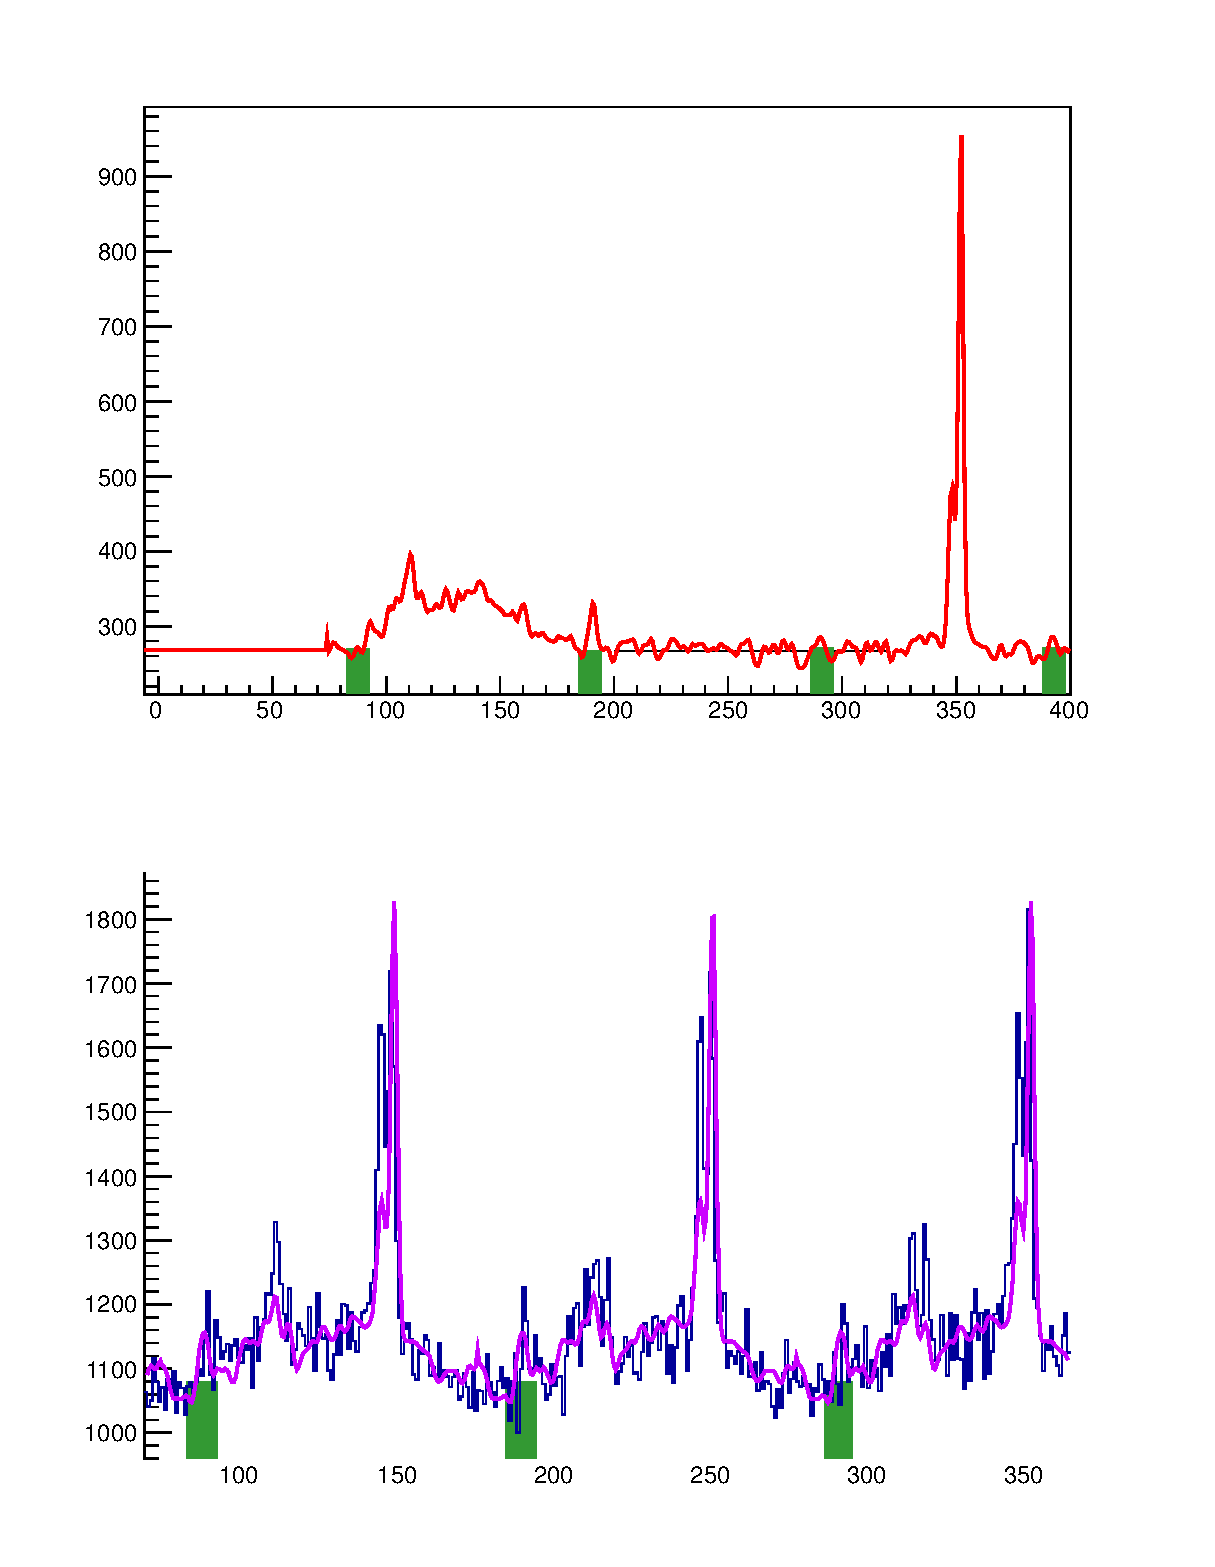
\includegraphics[width=0.8\textwidth]{figures/PDE_1.eps}
\caption{Extracting non-pulse-selected counts (below) using the pulse-selected data (above) to generate a fit.  Estimated background is shown in green.}
% make scales match
\label{fig:NPS_fits}
\end{figure}


\section{Placing a Limit on Excited \zp States}
\label{sec:zpLimit}
\begin{comment}
introduce 0+ peak and see when it becomes statistically significant
there will be different limits for different energies!  because of the evaporation background
\end{comment}
A primary aim of this experiment is to investigate the distribution of \zp strength, making it important to either measure or place a limit on the cross sections of excited \zp states.  Because the non-pulse-selected data has significant, complicated background, only the pulse-selected data sets were used for this analysis.  Because the \zp cross section is largest at forward angles, spectra from the three forwardmost detectors was summed to make the TOF spectrum used in this analysis.  These three detectors span lab angles 6.1$^{\circ}$ to 7.7$^{\circ}$.  The fourth detector, at 8.4$^{\circ}$, was not included because the \zp cross sections noticeably decline at this angle.  Including this detector or any detectors beyond it would have introduced background without contributing significant signal, worsening the sensitivity.    

% expand on states that were observed?
No obvious \zp states were observed above the neutron continuum for \Ge{74} or \Ge{76} targets.  A limit on the cross-section of \zp states as a function of energy can be determined by solving for the number of counts $S$ necessary to be consistent with zero within $i$ standard deviations $\sigma_S$:
\begin{equation}
S = P - B = i\sigma_S,
\end{equation}
where $P$ is the number of counts in the potential signal region and $B$ is an estimate of the counts in that same region.  In this case, sideband subtraction is the most appropriate method of determining $B$ because the shape of the continuum is not well-known and attempting to fit it functionally could introduce additional systematic error.  The error associated with the signal-induced counts $S$ is then
\begin{equation}
\sigma_S = i\sqrt{P+B} \approx i\sqrt{S+B+B} = i\sqrt{S+2B}.
\end{equation}
The number of signal counts $S$ can now be written as a function of the background counts $B$ and the desired level of certainty, $i$:
\begin{equation}
S = \frac{i^2 \pm \sqrt{i^4 + 8i^2B}}{2}.
\end{equation}
Note that the number of background counts $B$ scales with the chosen integration window.  The limits shown were calculated with an integration window of $\sim$7~ns, wide enough to include 95\% of the peak assuming its resolution is the same as that of the ground-state peak.

The $2\sigma$ limit on the cross-section for excited \zp states in \Ge{74} and \Ge{76} is shown in {\fig}~\ref{fig:zp_limit}.  The $2\sigma$ limit was chosen in order to have 95\% confidence in the existence of a peak.  A simulation of peaks at the 2$\sigma_S$ limit is shown in {\fig}~\ref{fig:differentLimits}.
\begin{figure}[!htbp]
\centering
\subfloat[][]{
   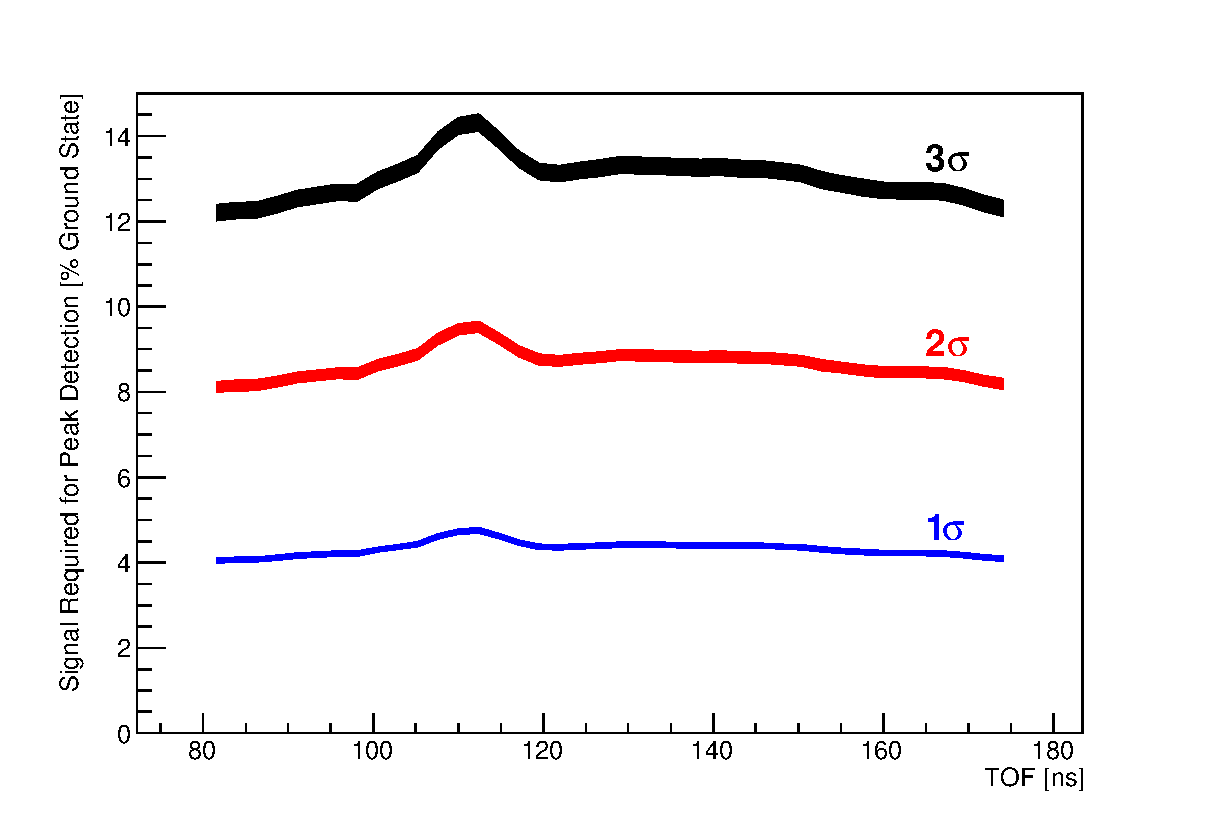
\includegraphics[width=0.45\textwidth]{figures/74Ge_limits.eps}
}
\hspace{8pt}
\subfloat[][]{
   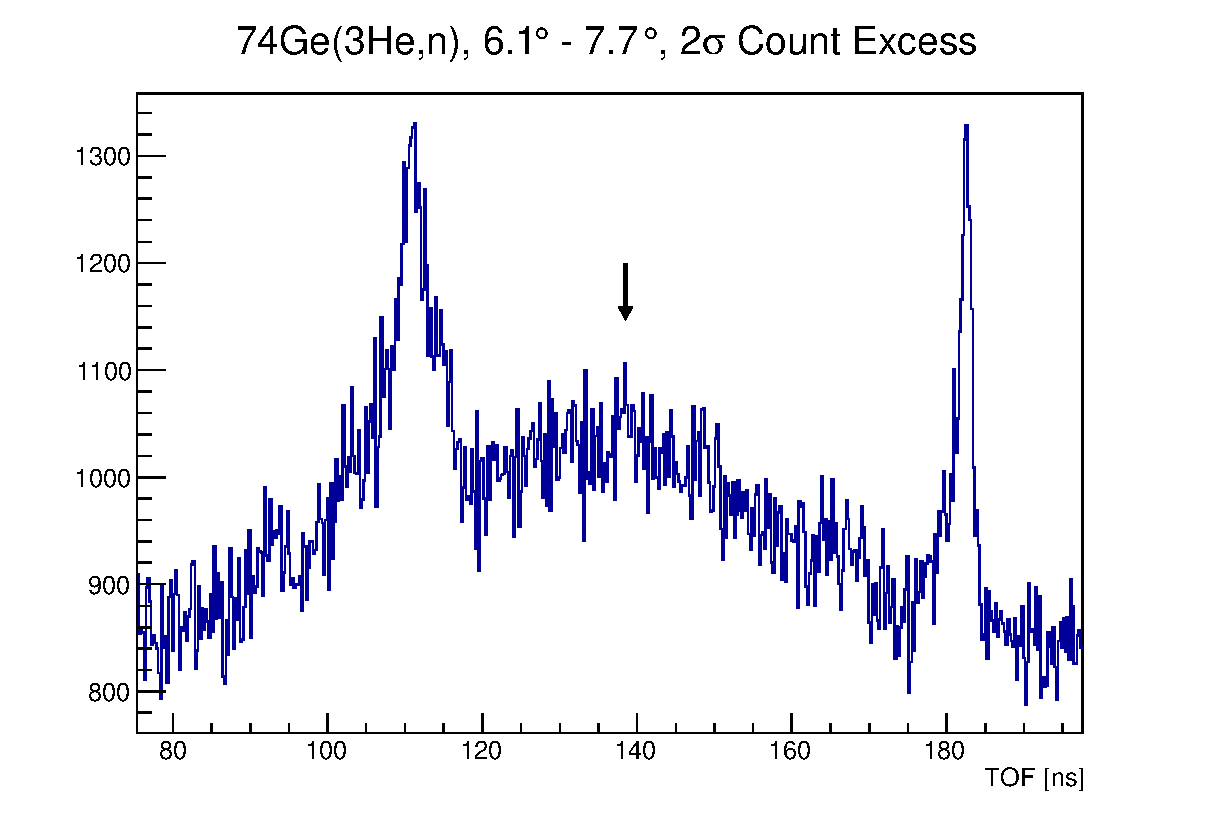
\includegraphics[width=0.45\textwidth]{figures/74Ge_2sigma_limit.eps}
} \\
\subfloat[][]{
   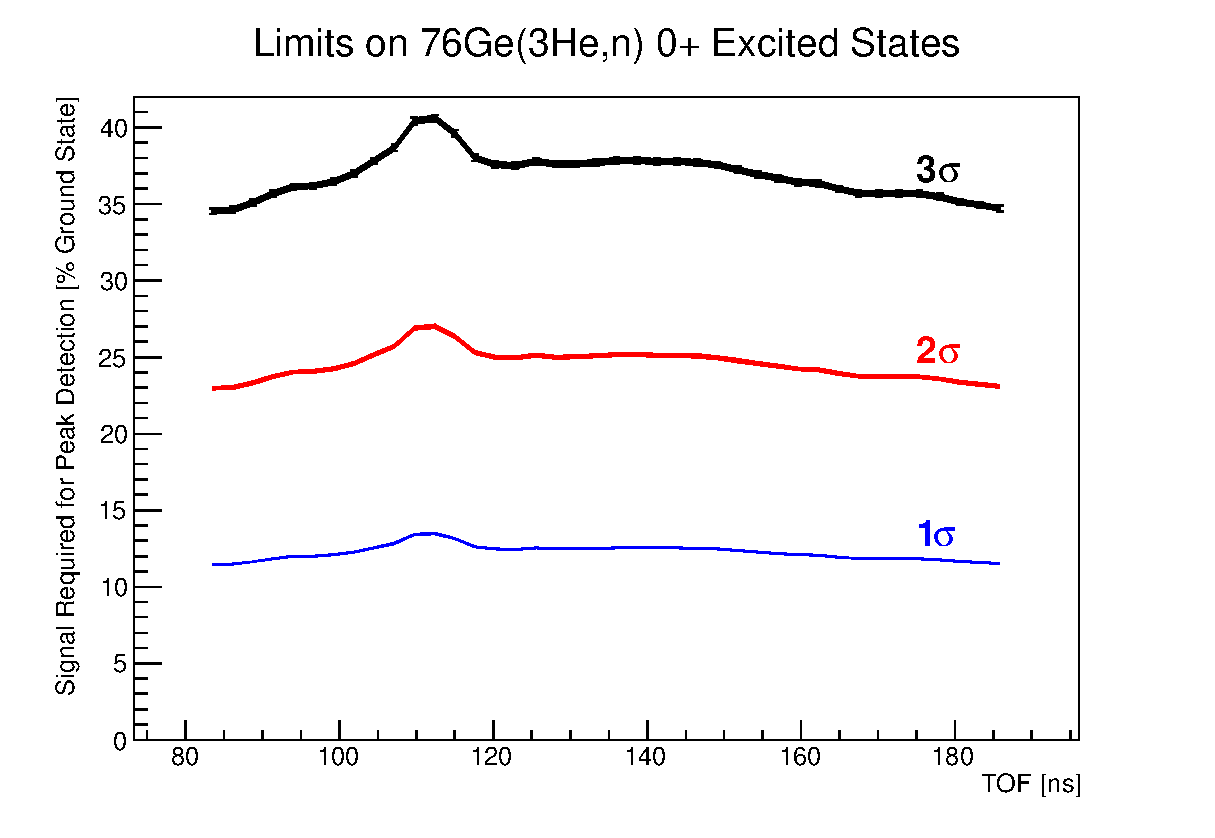
\includegraphics[width=0.45\textwidth]{figures/76Ge_limits.eps}
}
\hspace{8pt}
\subfloat[][]{
   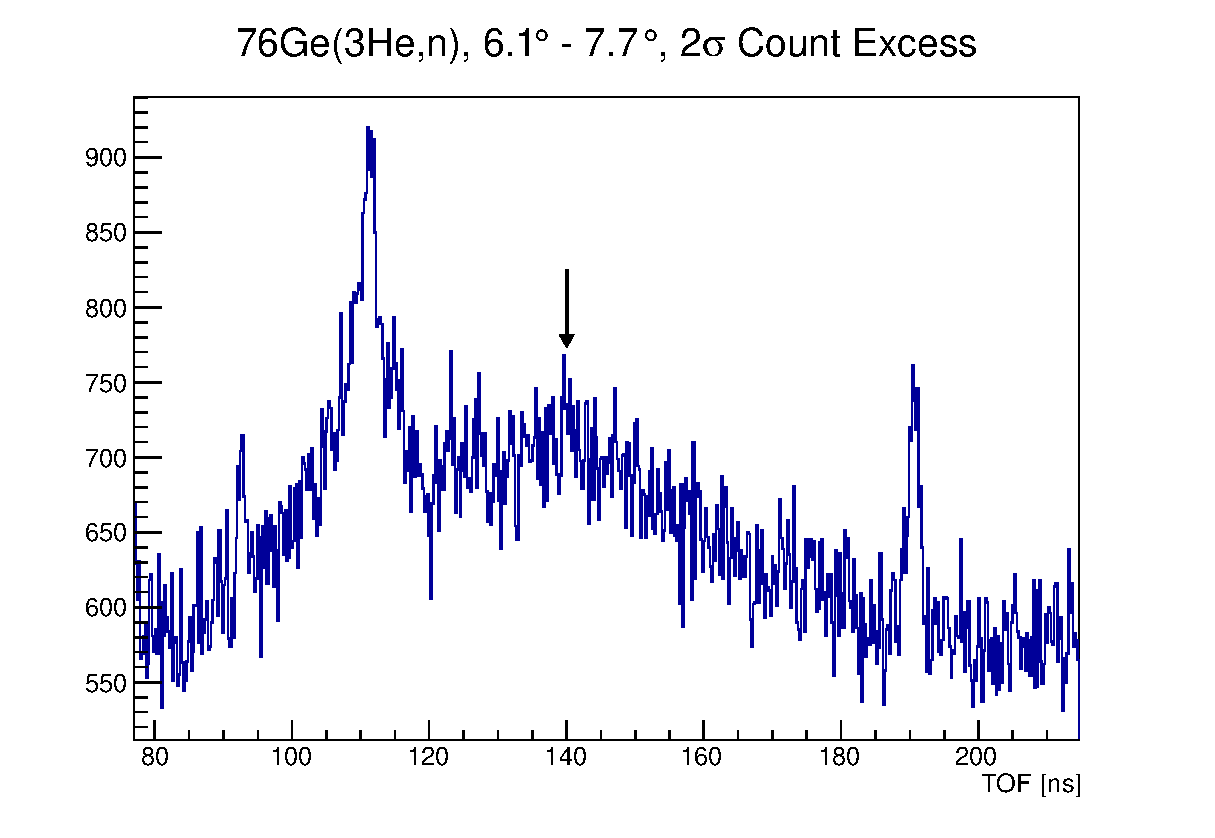
\includegraphics[width=0.45\textwidth]{figures/76Ge_2sigma_limit.eps}
}
\caption{Limit on excited \zp states as a percentage of the ground-state cross section for $^{74}$Ge (above) and $^{76}$Ge (below).  The thickness of the line indicates the error of the estimate.  The limit is poor for neutrons arriving at times less than 120~ns relative to the $\gamma$ peak because of the broad neutron peak due to oxygen contamination in the targets.  The effect of a signal with 2$\sigma$ significance is simulated for $^{74}$Ge (b) and $^{76}$Ge (d).}
% excitation energy, not timing
% don't show past big peak
\label{fig:differentLimits}
\end{figure}

\section{Fitting the \zp ground state}
\begin{comment}
DWBA calculation
shell model
f$^2$, p$^2$ state strength ("form factor")
\end{comment}
The ground-state cross section of $^{74}$Ge($^3$He,n)$^{76}$Se is nearly twice {not twice} that of $^{76}$Ge($^3$He,n)$^{78}$Se.  One may wonder if this is due to missing \zp strength.  One way to check whether this could be the case is by calculating the zero-degree cross section with a model that assumes the \zp strength to be in the ground state and comparing this to the measured values.  The measurement is not the zero-degree ground-state cross section, but rather the angular distribution of the ground and first excited state together. DWBA must be used to calculate the zero-degree ground-state cross section {say what you did: used ang dists to extrapolate}. Fresco [cite] was used to perform the DWBA calculations, which requires the binding potential for the di-proton in the \He{3} and \Ge{74} nuclei as well as the optical-model potentials experienced by the incoming \He{3} nucleus and the outgoing neutron.  Typical values for the parameters of these potentials are given in {\tab}~\ref{tab:typicalPotentials}, where the optical models used for the \He{3} and neutron are Becchetti-Greenlees [CITE] and Koning-Delaroche [CITE], respectively.  The results of the fit to the measured angular distributions are shown in {\fig}~\ref{fig:PS_angularDistribution}.
\begin{table*}\footnotesize
\caption{\label{tab:typicalPotentials} Optical and bound-state potentials used in the DWBA analysis, see the text for details of the calculations. Both optical potentials vary slowly with $N$, $Z$ and $E$; the values given here are typical. $^{\dagger}$ Adjusted to reproduce the experimentally measured binding energy.}
%\begin{ruledtabular}
\begin{tabular}{ccccccccccccccccc}
\hline
Particle & V & r & a & V$_{\text{SO}}$ & r$_{\text{SO}}$ & a$_{\text{SO}}$ & W & r$_{\text{W}}$ & a$_{\text{W}}$ & W$_{\text{D}}$ & r$_{\text{WD}}$ & a$_{\text{WD}}$ & W$_{\text{SO}}$ & r$_{\text{WSO}}$ & a$_{\text{WSO}}$ & r$_{\text{c}}$ \\
\hline
$^{3}$He & 157.1 & 1.20 & 0.72 & 2.50 & 1.20 & 0.72 & 43.4 & 1.40 & 0.88 & - & - & - & - & - & - & 1.30\\
n & 45.27 & 1.21 & 0.54 & 5.57 & 1.03 & 0.59 & 1.18 & 1.21 & 0.54 & 6.76 & 1.34 & 0.53 & -0.07 & 1.03 & 0.59 & -\\
$^3$He bound state & 76.6 & 1.175 & 0.65 & - & - & - & - & - & - & - & - & - & - & - & - & 1.30\\
Se bound state & 100$^{\dagger}$ & 1.30 & 0.65 & - & - & - & - & - & - & - & - & - & - & - & - & 1.30\\
\hline
\end{tabular}
%\end{ruledtabular}
\end{table*}
% and now the figure
% put table sideways and combine with other table
\begin{figure}[!htbp]
\centering
\subfloat[][]{
   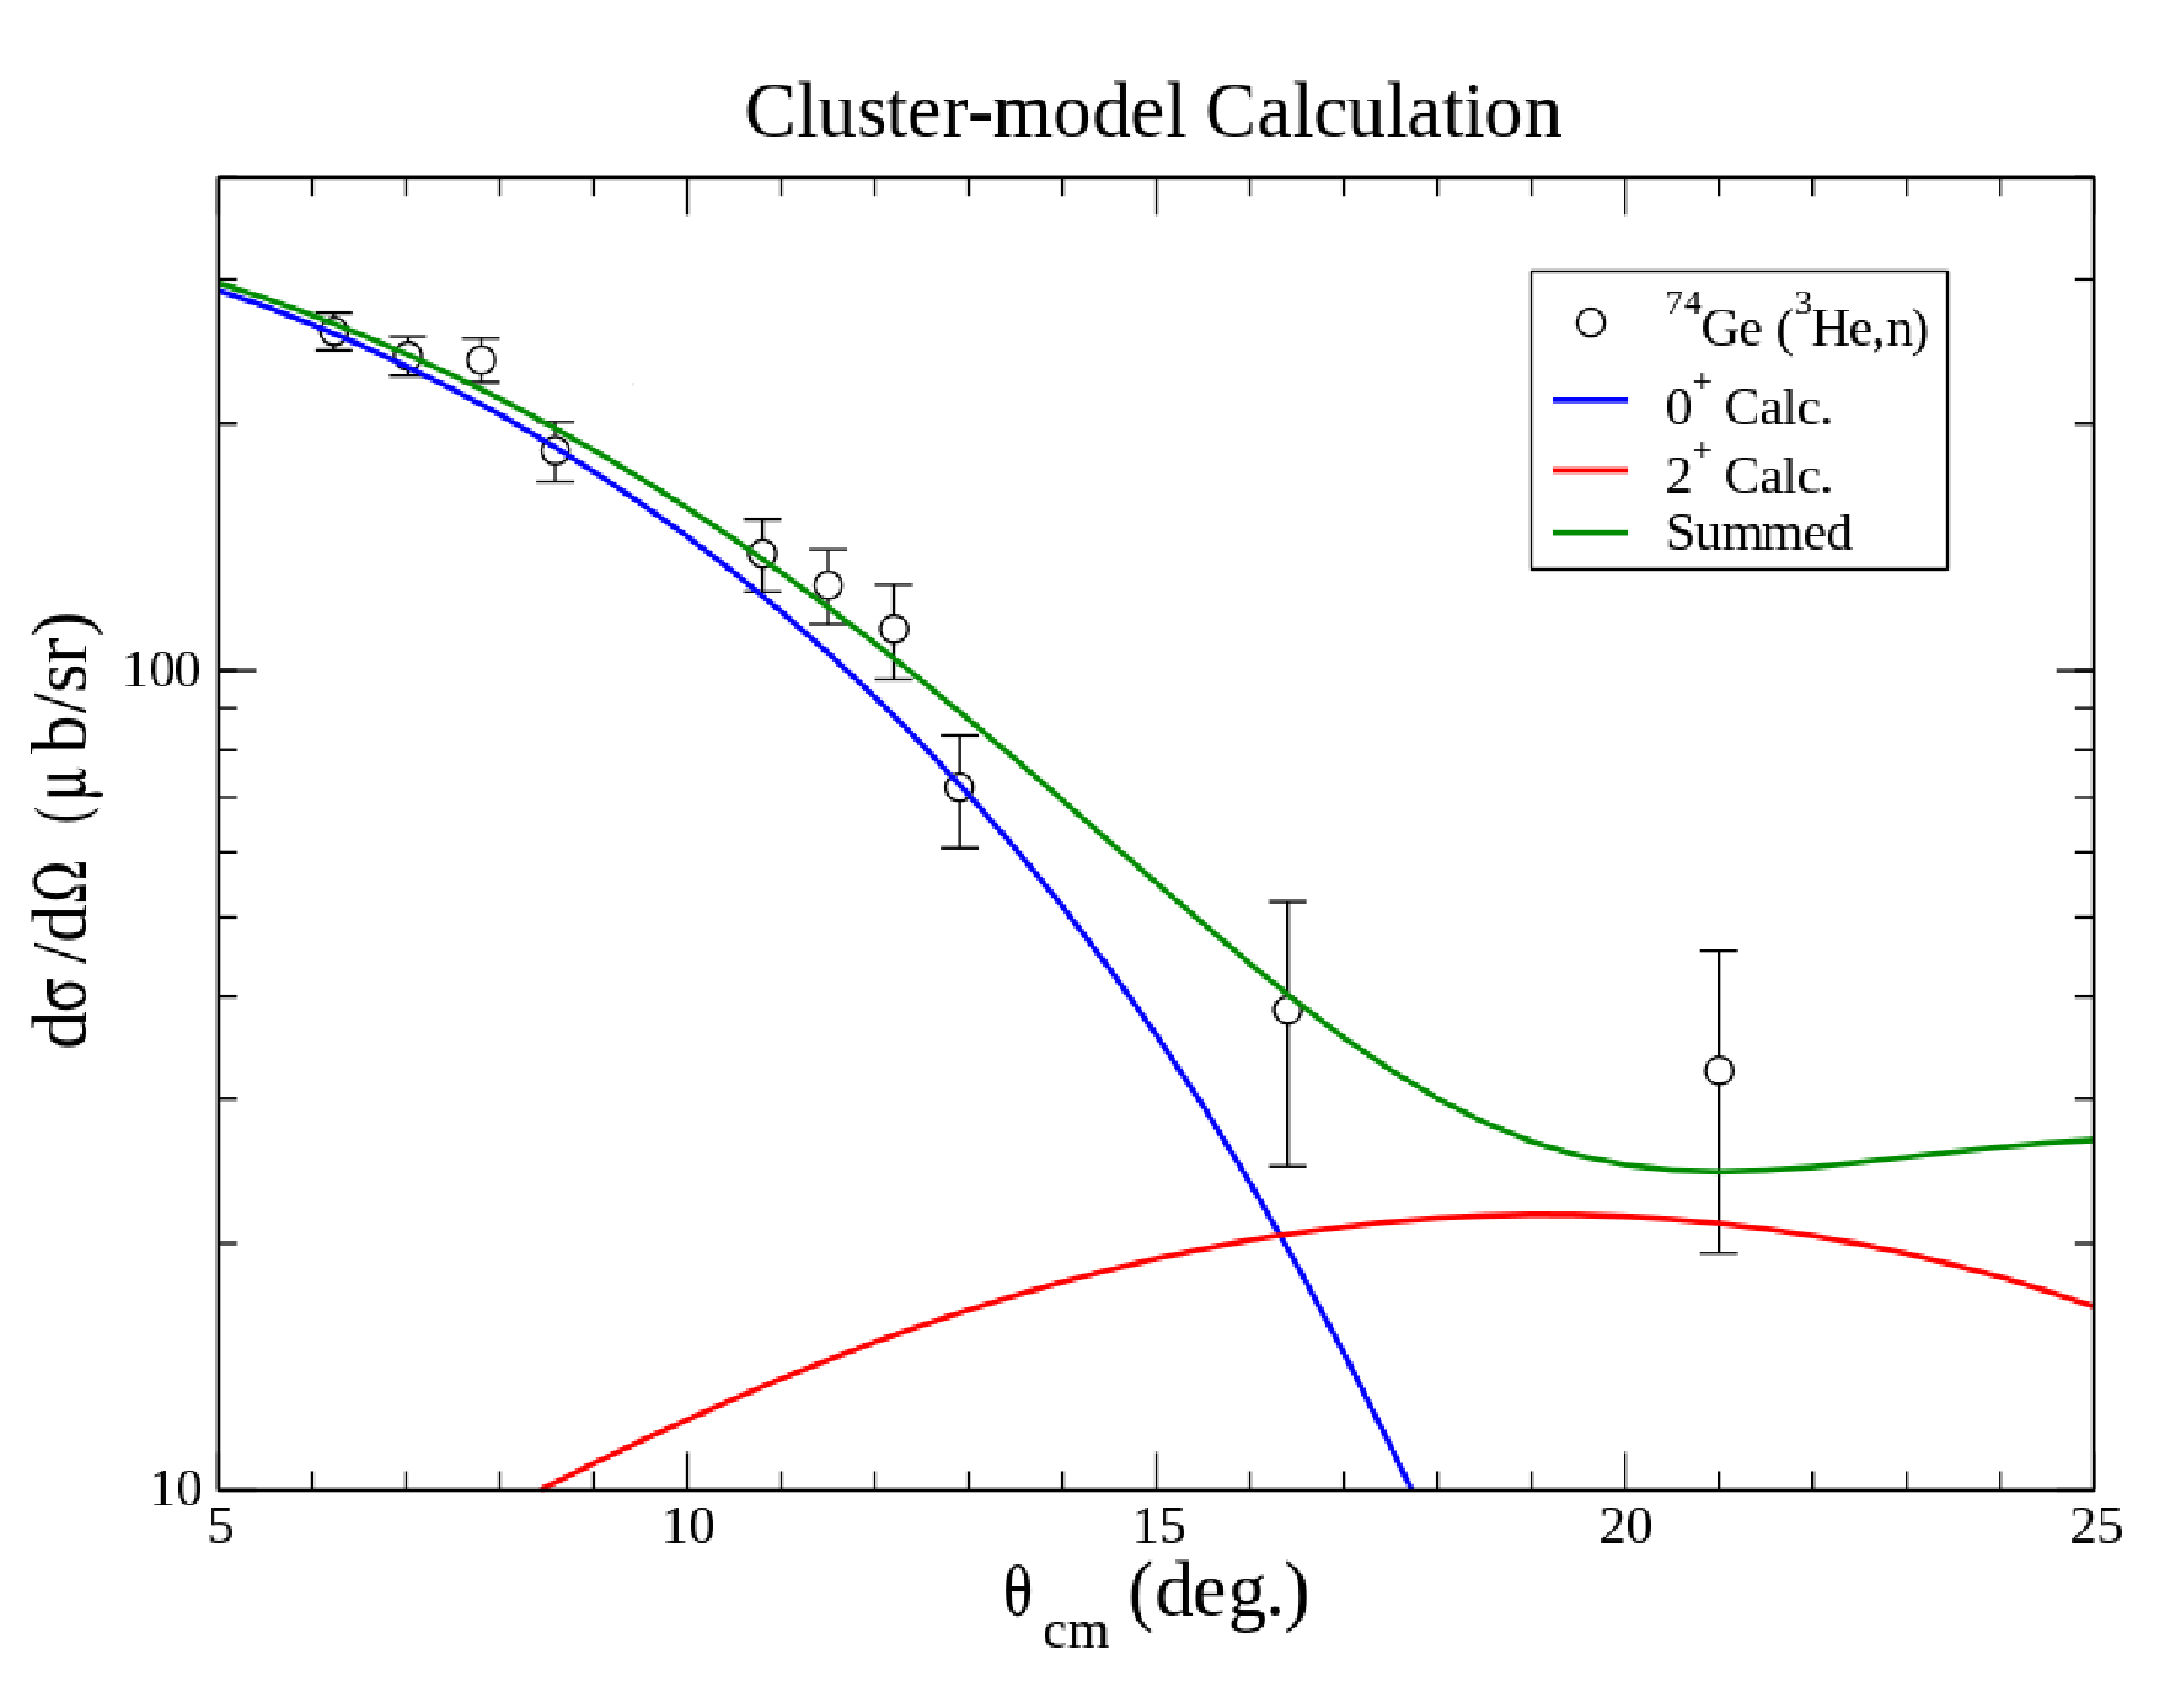
\includegraphics[width=0.5\textwidth]{figures/74Ge_angularDist.eps}
}
\subfloat[][]{
   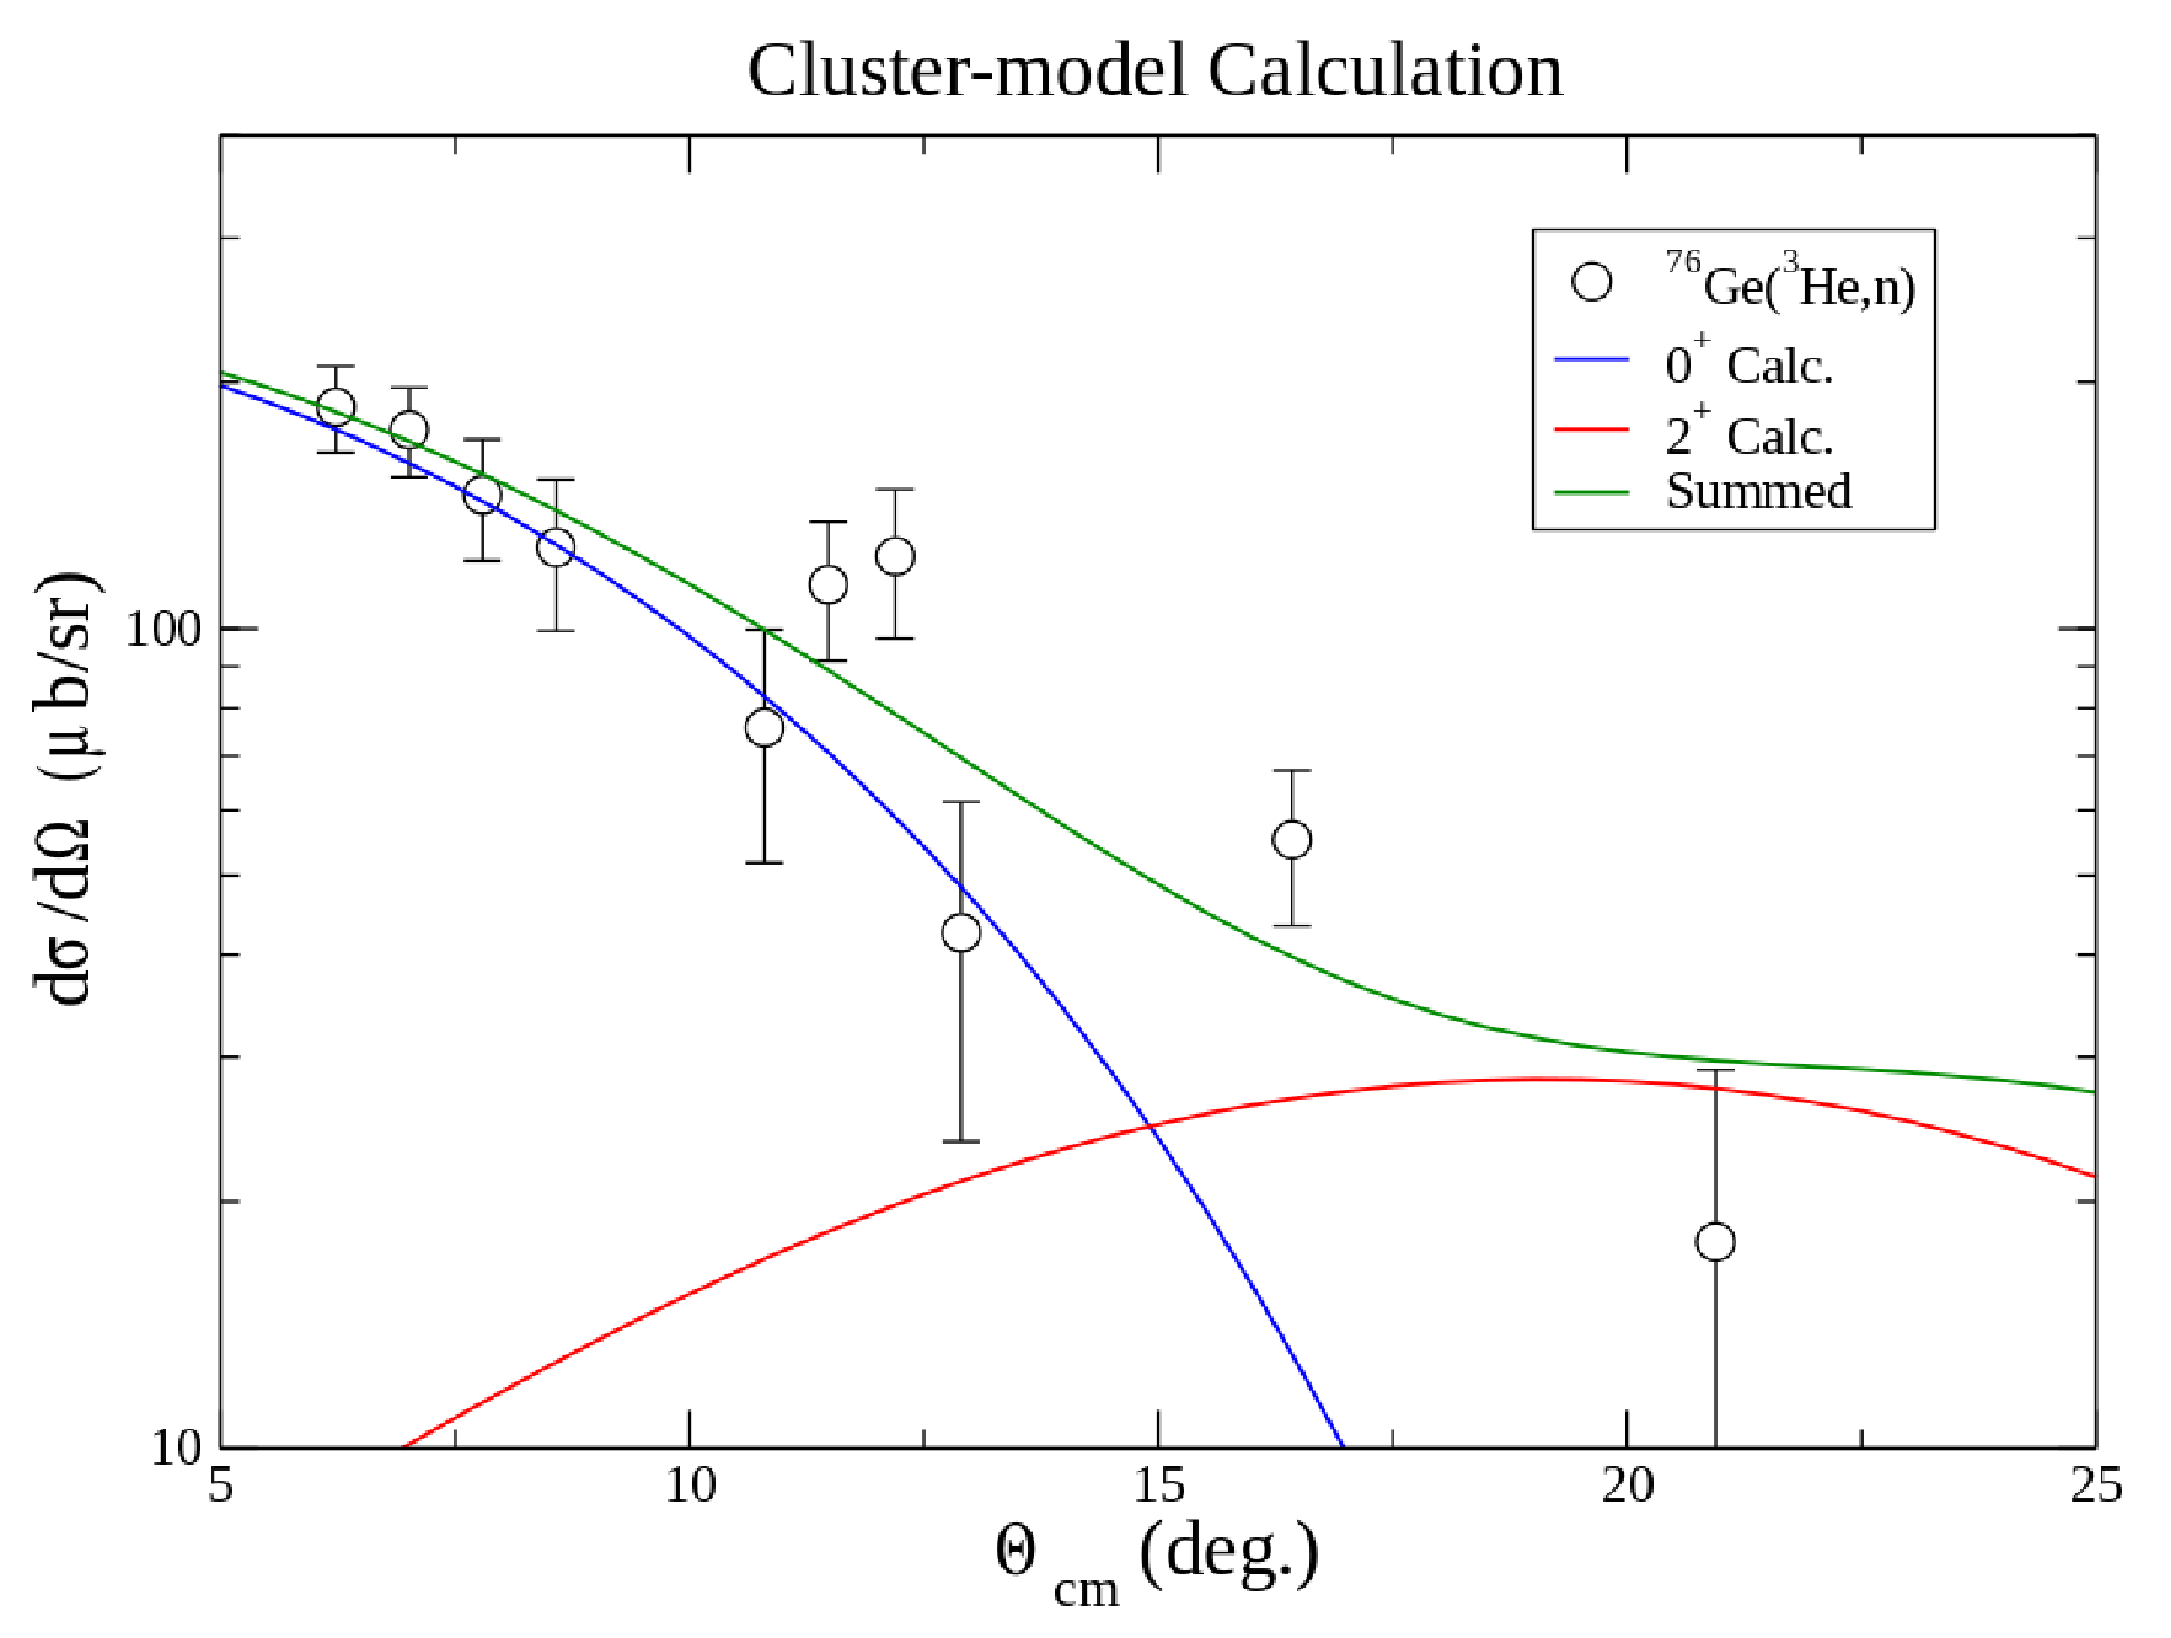
\includegraphics[width=0.5\textwidth]{figures/76Ge_angularDistribution.eps}
}
\caption{The angular distributions of $^{74}$Ge($^3$He,n)$^{76}$Se (a) and $^{76}$Ge($^3$He,n)$^{78}$Se (b).  In each graph, the two back-angle measurements are four-bar averages.  Because the timing resolution did not allow clear separation of the ground and first excited states, the integration window included both.  The data are well-described by the sum of the two states.}
\label{fig:PS_angularDistribution}
\end{figure}
 
The cluster model is sensitive to the parameters used to describe the potentials of the interacting nuclei.  The sensitivity of the extracted zero-degree cross section on the bound-state radius parameter, the neutron optical-model potential, and the principal quantum number were all investigated.  While changing the bound-state radius strongly affects the normalization, it does not appreciably affect the shape of the angular distribution between 0$^{\circ}$ and 20$^{\circ}$ and therefore does not impact the ratio of ground-state to first-excited-state cross section at zero degrees.  Using the Becchetti-Greenlees neutron potential rather than the Koning-Delaroche petential does not strongly affect the angular distribution, nor does changing the principal quantum number.  The effect of varying these parameters is shown in {\fig}~\ref{fig:varyParam}.
\begin{figure}[!htbp]
\centering
\includegraphics[width=0.8\textwidth]{figures/AngDist.eps}
\caption{Sensitivity of angular distributions on bound-state radius, neutron potential, and principal quantum number.  All calculations are normalized to 350~$\mu$b/sr at zero degrees.}
\label{fig:varyParam}
\end{figure}
 The dependence of the cross-section for various \He{3} optical potential models was also explored and found to result in little difference in the trend in the zero-degree cross sections of \Ge{74} and \Ge{76}.  See {\tab}~\ref{tab:parameterSensitivity} for the tested parameter ranges and {\fig}~\ref{fig:parameterSensitivity} for their impact on the relative cross-section.
\begin{table}[htp]
\centering
\begin{tabular}{lll}
 & DGP08 & Urone \\
\hline
$V_0$ (MeV) & 118.3 & 175.4 \\
$r_R$ (fm) & 1.30? & 1.14 \\
$r_C$ (fm) & 1.24 & 1.4 \\
$a_R$ (fm) & 0.82? & 0.71 \\
W (MeV) & 34.2? & 19.9 \\
$r_l$ (fm) & 1.31? & 1.53 \\
$a_l$ (fm) & 0.84? & 0.85 \\
$W_D$ (MeV) & 106.4? & 9.13(N-Z)A \\
Norm. Factor & 0.904 & 0.910 \\
\end{tabular}
\caption{Optical parameters used for three different models of the \He{3} potential.}
\label{tab:parameterSensitivity}
\end{table}

\begin{figure}[!htbp]
\centering
\includegraphics[width=0.8\textwidth]{figures/CrossSectionVsN_ElasticSurvey.eps}
\caption{The GDP08 potential differs from the Becchetti and Urone potentials for nickel and strontium isotopes, but all potentials reproduce the measured Q-value dependence of \GeTargets.  The calculations are normalized to the \Ge{74} data.}
\label{fig:parameterSensitivity}
\end{figure}

As discussed in {\chap}~\ref{chap:nucl}, both the Cluster and Bayman-Kallio models typically describe the same shape for the $L=0$ angular distribution, but neither model typically reproduces the absolute cross-section.  In the case of the $^{58,60,62,64}$Ni and $^{88}$Sr isotopes, however, the Cluster model reproduces the trend as a function of the neutron number rather well.  This agreement is shown in {\fig}~\ref{fig:nickelTrend}, where all cross-sections have been normalized to $^{58}$Ni.  
\begin{figure}[!htbp]
\centering
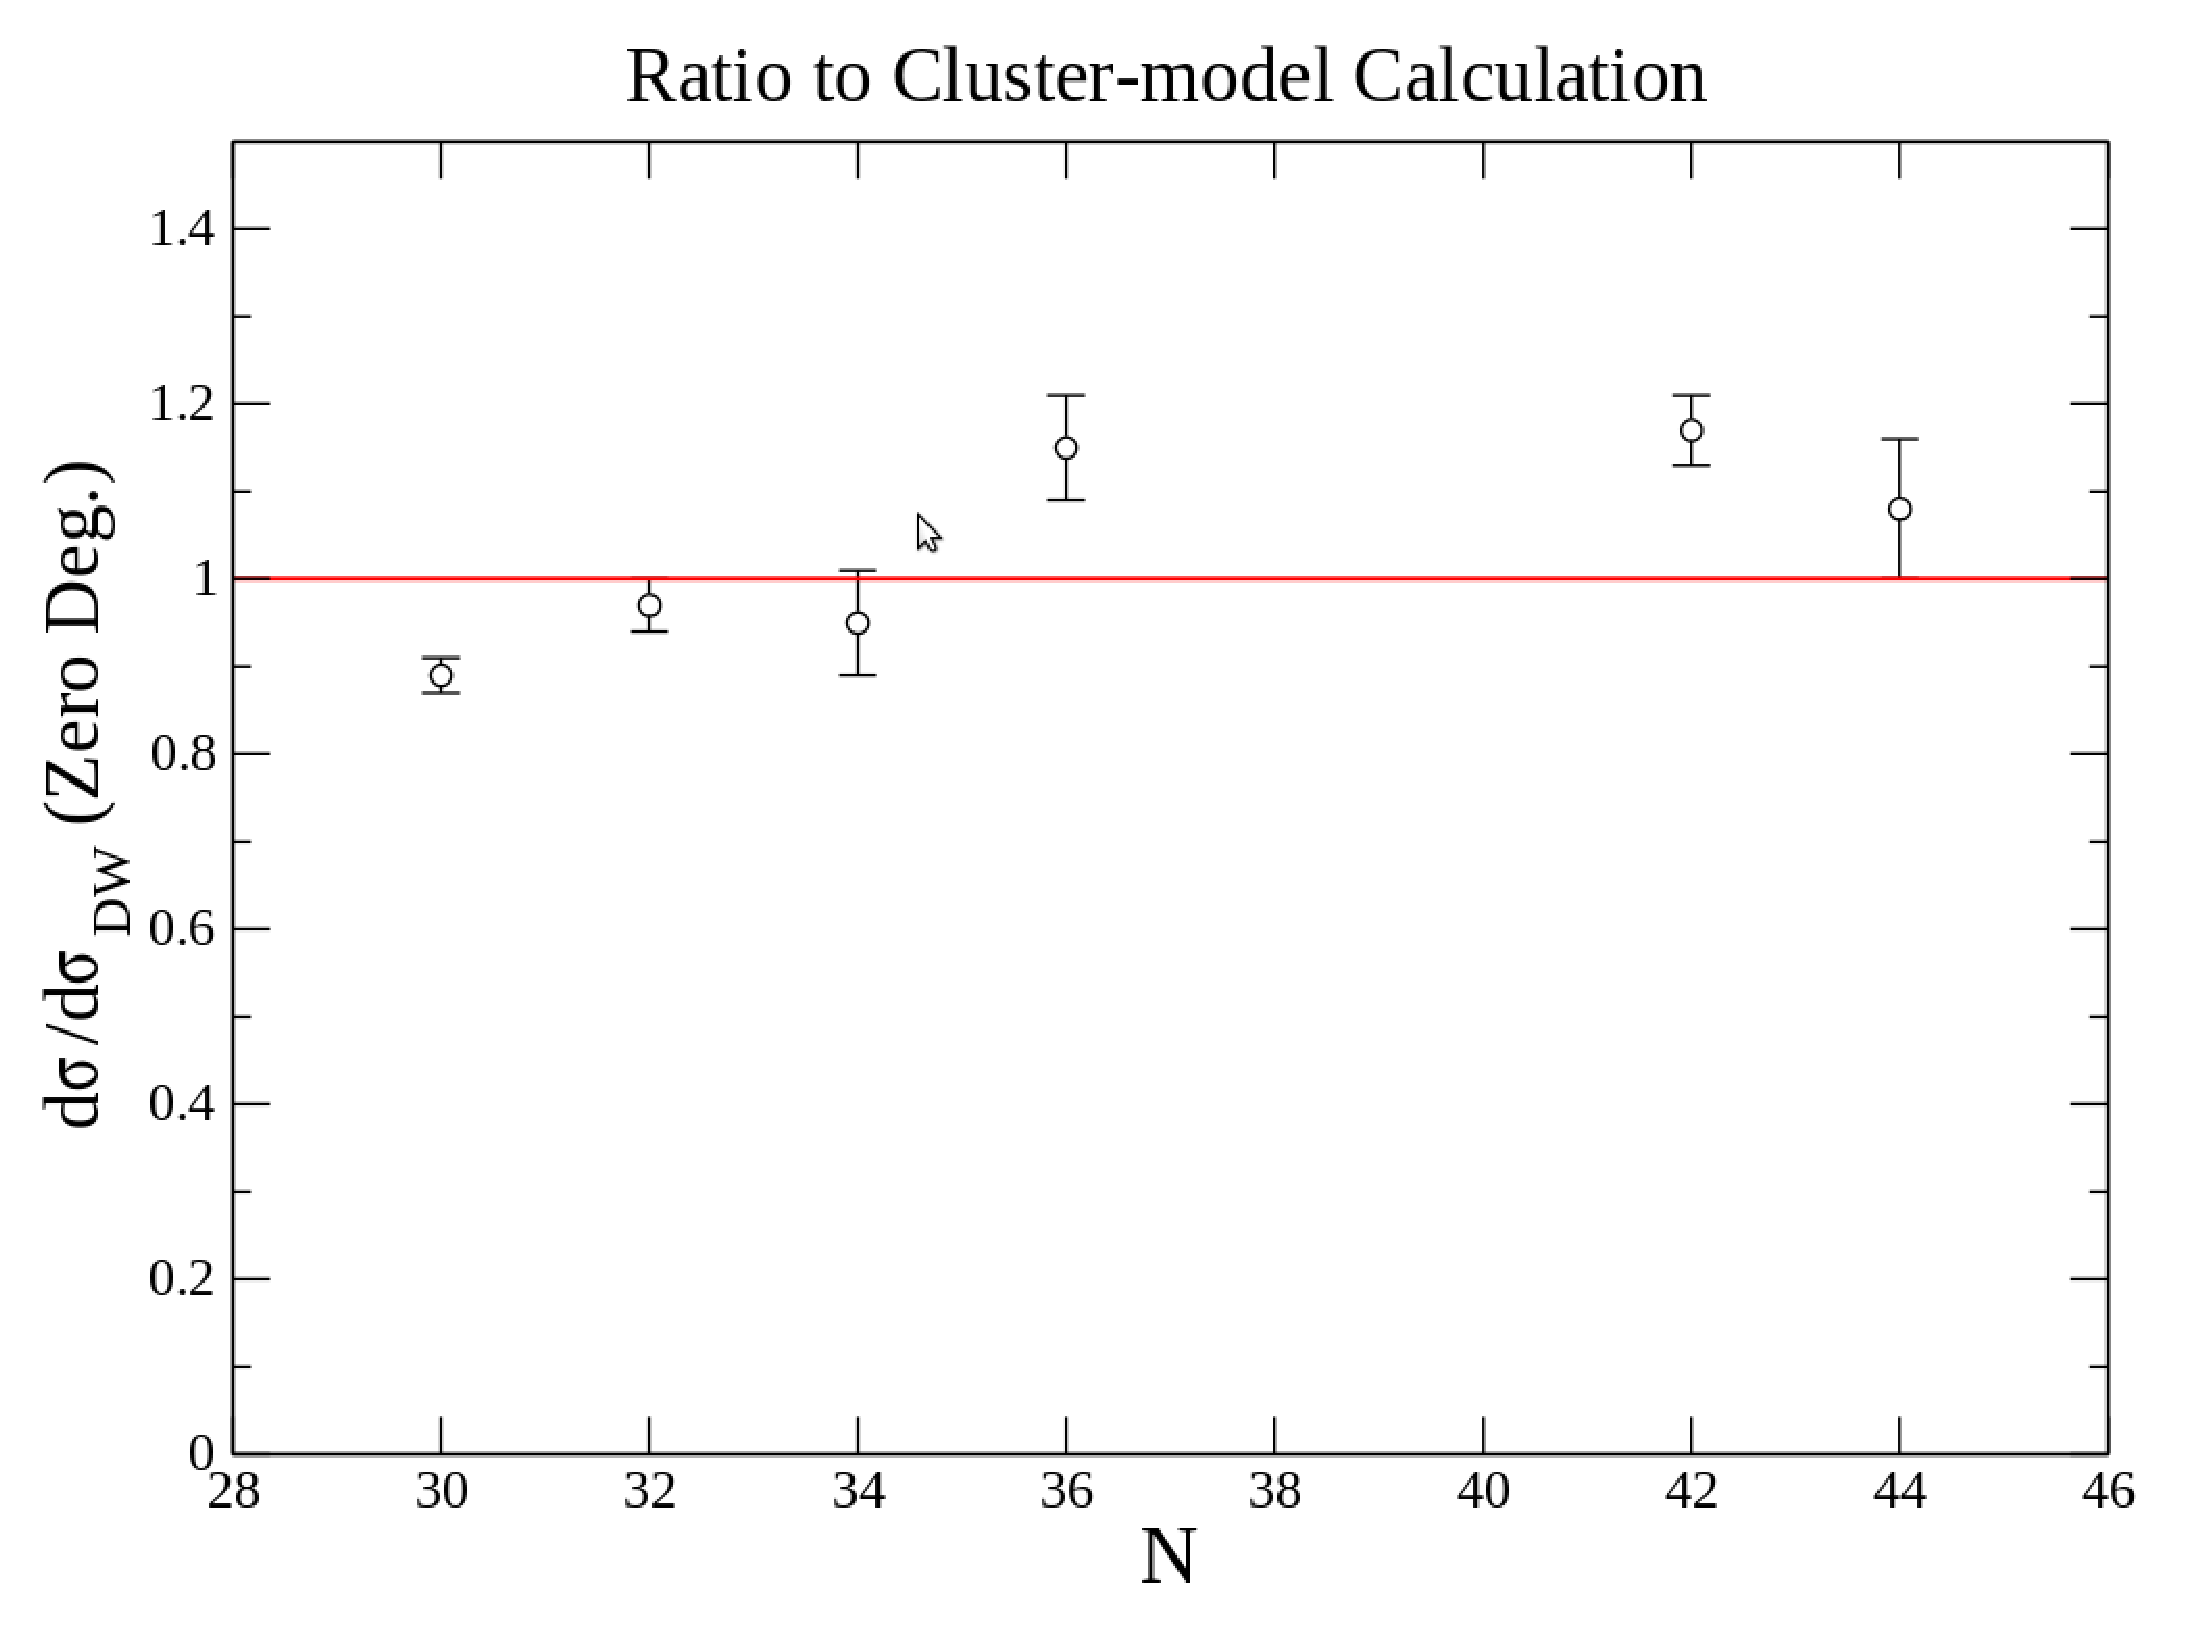
\includegraphics[width=0.8\textwidth]{figures/nickel_trend.eps}
\caption{The cluster model describes the trend for Ni and Ge isotopes.  The cross-sections are normalized to the best fit.}
\label{fig:nickelTrend}
\end{figure}
The cluster model, then, accurately describes the trend when adding protons to f-p-g shell nuclei in this mass region.  Cluster model calculations of the $^{74}$Ge($^3$He,n)$^{76}$Se and $^{76}$Ge($^3$He,n)$^{78}$Se reactions show that the smaller cross section of the $^{76}$Ge($^3$He,n)$^{78}$Se reaction is likely due to the Q-value dependence reproduced by DWBA and probably not due to ground-state loss of \zp strength.   The cross-sections measured for \reaction are consistent with DWBA predictions and the data suggest no significant excited \zp states.

% % uncomment the following lines,
% if using chapter-wise bibliography
%
% \bibliographystyle{ndnatbib}
% \bibliography{example}
